%\documentclass[11pt]{book}
\documentclass[10pt]{article}
%\documentclass[11pt]{amsart}
%\documentclass[preprint,12pt]{elsarticle}

\usepackage{etex}
\usepackage{standalone}
\usepackage{tikz}
% !TEX root=img/arguments_and_attack.tex

% \usetikzlibrary{external} 
% \tikzexternalize[prefix=tikz/] 

\usetikzlibrary{calc}
\usetikzlibrary{arrows}
\usetikzlibrary{arrows.meta}
\usetikzlibrary{decorations.markings}
% \usetikzlibrary{intersections}
\usetikzlibrary{fit}
\usetikzlibrary{shapes}
% \usetikzlibrary{trees}


\tikzset{
	every path/.style={thick},
	align=center,
	observed/.style={
		fill=black!20,
	},
	bn/.style={
		draw,
		ellipse,
		-{Triangle[angle=60:6pt 0]}
	},
	scn/.style={
		draw,
		rectangle,
		% signal,
		% signal from=west,
		% signal pointer angle=120,
		-{Triangle[angle=60:6pt 0]},
	},
	possibly/.style={dashed},
	arg/.style={
		draw,
		rectangle,
		-{Straight Barb[angle=60:6pt 0]}
	},
	attack/.style={
		-{Rays[width=10pt,length=10pt,sep=-3.9pt]}
	},
	pref/.style={
		draw,
		rectangle,
		-{Straight Barb[angle=60:6pt 0]}
	},
	subscn/.style={
		double,
		-{Triangle[angle=60:6pt 0]},
	},
	specific/.style={
		double,
		-{Stealth[angle=60:6pt 0]}
	},
}



%tikz
\usepackage{dcolumn}
\usepackage{booktabs}
% \usepackage{tikz}
\usetikzlibrary{positioning,shapes,arrows}
\newcolumntype{M}[1]{D{.}{.}{1.#1}}

%images
\usepackage{subcaption}
\usepackage{graphicx}

\usepackage{multirow}
\usepackage[all]{xy}
\usepackage{verbatim} 
\usepackage{endnotes}
\usepackage{amssymb} 
\usepackage{setspace} 
%\doublespacing
\onehalfspacing
%\usepackage{mathabx}
\usepackage{amsmath}
\usepackage{hyperref} % for urls
\hypersetup{pdfborder={0 0 0}}

%\usepackage{diagrams}

%\usepackage{bookman}
%\usepackage{helvet}
\usepackage{palatino}
%\usepackage{times}


%\usepackage{charter}
%\usepackage{avant}
%\usepackage{chancery}
%\usepackage{utopia}

\def\setgrouptext#1{\gdef\grouptext{#1}}
\newenvironment{groupeditems}{\begin{displaymath}\left.\vbox\bgroup\setgrouptext}{%
  \egroup\right\rbrace\hbox{\grouptext}\end{displaymath}}
  
\usepackage{fancyhdr}

%\pagestyle{fancy}

\usepackage{sectsty}
%\allsectionsfont{\sffamily} 
\chapterfont{\Large \scshape}
\sectionfont{\large \scshape \centering}
\subsectionfont{\normalsize \itshape}
%\subsectionfont{\large \nohang \flushleft} 
%\allsectionsfont{\mdseries\itshape} 
%\sectionfont{\fontfamily{ptm}\selectfont}

% \usepackage{fullpage}


\usepackage[margin=1.5in]{geometry}

\usepackage{lastpage}

\usepackage{fancyhdr}
\setlength{\headheight}{15.2pt}
\pagestyle{fancy}

%\rhead[<even output>]{\textsc{\large Dissertation Summary} --  \thepage \textit{ of}   \pageref{LastPage}}
\rhead[<even output>]{\textsc{\small Evidential Reasoning} -- \ \thepage \textit{ of}   \pageref{LastPage}}
%\chead[<even output>]{<odd output>}
\lhead[<even output>]{\text{\small Di Bello \& Verheij}}

%\lfoot[<even output>]{<odd output>}
\cfoot[<even output>]{}
%\rfoot[<even output>]{ \thepage \textit{ of}   \pageref{LastPage}}




\usepackage{pgfplots}
\pgfplotsset{compat=1.13}
 
\usepackage[round]{natbib}
\begin{document}

\thispagestyle{empty}

\vspace{-2cm}
\noindent
%\section*{ \hspace{6cm} \Large DRAFT - begin}
-----------------------------------------------------------------------------------------------------------------------
%\section*{ \Large Writing Sample A}


\vspace{5mm}
\noindent
\textsc{\large \bf  EVIDENTIAL REASONING \\ Chapter for the Handbook of Legal Reasoning}

\vspace{3mm}
\noindent
Marcello Di Bello \& Bart Verheij --  \today \\
%Word count:  9723.
\vspace{1cm}

\vspace{1cm}



\vspace{1cm}

%\begin{abstract}
%mmm
%\end{abstract}

%QUESTION: WILL THIS BE A "US CENTRIC" CHAPTER? I HATE THAT, BUT I AM AFRAID MY PART WILL BE US CENTRIC. 

\tableofcontents

\newpage

\noindent When a suspect appears in front of a criminal court, there is a very high probability that he will be found guilty. In the Netherlands, for instance, the conviction rate of suspects that appear in criminal courts is reported to be around 95\% year after year.\footnote{Source: CBS, the Dutch central bureau of statistics, publishing its data at www.cbs.nl.} [NOT SURE ABOUT THE DUTCH FIGURE BEING FIRST]In the United States, the conviction rate in federal courts has been roughly 75\% and in Japan it has reached as high a rate as 99\%.\footnote{\textbf{SOURCE TO BE ADDED}} This does not mean that fact-finders deciding about the facts of a criminal case have an easy job. Whether laypeople, such as jury members selected from the general public, or professionals, often experienced judges having completed postgraduate education, all face the difficulties associated with handling the evidence that is presented in court. What to do with conflicting testimonies? Does an established DNA match outweigh the testimony that the suspect was not on the crime scene? How to coherently interpret a large body of evidence? What to do with illegally obtained evidence? [WE DO NOT ADDRESS THIS QUESTION IN THE TEXT, SO REMOVE?] When is there enough evidence to convict `beyond a reasonable doubt'? 

The primary aim of this chapter is to explain the nature of evidential reasoning, the characteristic difficulties encountered, and the tools to address these difficulties. Our focus is on evidential reasoning in criminal cases. There is an extensive scholarly literature on these topics, and it is a secondary aim of the chapter to provide readers the means to find their way in historical and ongoing debates. Before diving into the literature [THE CHAPTER IS NOT EXACTLY LITERATURE FOCUSED, SO MAYBE "DIVIDING INTO THE TOPIC?"], we set the stage by using two important and often encountered kinds of evidence as an illustration: eyewitness testimony and DNA profiling. Similarities and differences between these kinds of evidence are used to establish a list of central questions that structure the exposition that follows.

%\subsection{Setting the stage: eyewitness testimony and DNA profiling}

\section{Setting the stage}


Fact-finders---typically jurors and judges---aim to reconstruct what has happened in the crime on the basis of the evidence. 
We will use two central types of evidence to develop a list of central questions associated with evidential reasoning: eyewitness testimony and DNA analysis.

\subsection{Eyewitness testimony}

Eyewitness testimony has always been a central source of information in criminal proceedings. It typically takes the form of oral statements by the witness in court, in response to questions by the prosecution, the defense, the court, and sometimes, albeit rarely, the jury. Eyewitness testimony can also come 
in the form of written reports of oral examinations in the pre-court stages of the criminal investigation, normally by prosecuting officers and judges. 

Eyewitness testimony can provide detailed information about what has happened on the scene of the crime. Here is an example.
%
\begin{quote}
Q: Can you describe what happened, that day?

A: I was in the park and suddenly heard a lot of noise, very close by. I saw two men quarreling, shouting. Suddenly one of them pulled a gun, and I heard a shot. The other man fell to the ground. The shooter looked around, looked me in the eye, and then started to run.

Q: Can you describe the shooter?

A: He was a young men, in his twenties, I think. Tall, blonde, with a very white skin, and unusually blue eyes. He looked unhealthy, with bad teeth, 
like a drug addict. He was wearing an FC Groningen t-shirt, which surprised me as we were in the Vondelpark. [THIS REFERENCES TO GRONINGEN AND VONDELPARK, WHILE GOOD TO ILLUSTRATE THE IDEA OF SPECIFICITY OF THE TESTIMONY, WILL BE OBSCURE TO MOST READERS]
\end{quote}
%
On the basis of eyewitness testimony, we can form a hypothesis about what has happened. Sometimes this hypothesis contains specific detail---as in the example---, still it remains a hypothesis. 
[NOT SURE , STYLISTICALLY,  ABOUT THE COMMA AFTER THE DASH ---,]There are many reasons why the hypothetical events reconstructed on the basis of the testimony may not be true. Typical reasons against the truth of the events reported by an eyewitness include that a witness has wrongly interpreted what he saw, that time has distorted his memories, or that the witness is intentionally lying. 

\subsection{DNA profiling}

DNA profiling has become an important tool in courts. DNA profiling has a strong scientific underpinning, and comes with precise statistical information. The evidential relevance of a DNA profile stems from the fact that, although most of the structure of DNA is shared among all human beings (more than 99\%), the variations that do exist are very specific for each individual. 

A profile is determined by analyzing a number of specific locations---the so-called loci---of a DNA molecule, and establish the type of structure found there. These types are called alleles, and typically consist of the number of repetitions of a small DNA structure at a location. For instance, one locus used in the profiles stored in forensic DNA databases in the USA is referred to as CSF1PO, and it can have alleles 5, 6, 7 and then up to 16, depending on how often the molecular sequence AGAT is repeated at that location.\footnote{See \url{http://www.cstl.nist.gov/strbase/str\_CSF1PO.htm.}} Different countries use different sets of---what are called---core loci for their forensic DNA profile databases. [TERMINOLOGY IS NOT EXPLAINED HERE. WHAT ARE LOCI? WHAT ARE ALLELES? TABLE TO BE ADDED MIGHT HELP] For instance, the USA CODIS system has 13 core loci. As said, each specific DNA profile is rare, and reference databases of profiles 
are used to numerically measure how rare a profile really is [NOT SURE IF THIS IS ABOUT HOW RARE PROFILES REALLY ARE, BUT IT'S MOSTLY 
ABOUT ESTIMATING RARITY ON THE BASIS OF VALID MODELS]. This is done by counting the number of occurrences of each allele at each core locus in the reference database, which gives an estimate of the proportional frequency of that allele at that locus in the population. The measured proportional frequencies for the individual alleles at the core loci are then multiplied to compute what is called the Random Match Probability of the DNA profile.\footnote{Some special care is needed to accommodate for the fact that an allele can be from either part of the double helix that comprises our DNA.} These Random Match Probabilities---and numbers mathematically related to them---are the numbers reported by forensic experts in courts, and the smaller they are, the higher the evidential value of the profile is taken to be. The sets of core loci have been chosen such that Random Match Probabilities are typically very small, for instance, in the order of 1 in 50 billion, amply exceeding the number of people on our planet. The use of more loci leads to smaller Random Match Probabilities. A key assumption underlying the model (used when multiplying the estimated probabilities of specific alleles) is that there are no dependencies among the alleles at different loci in the population considered. This assumption does not always hold, for instance in a population with family relations. Scientists have also established certain dependencies among the profiles within ethnic groups. Moreover, testing the independence assumption can be hard, and require the assessment of more profiles than reasonably possible. [BUT I THINK THERE IS LITERATURE THAT HAS TESTED THE INDEPENDENCE ASSUMPTION. DO WE MENTION IT? BUCKLETON BOOK?]

Suppose now that a trace of blood has been found on the scene of the crime, and that the found DNA profile matches that of the suspect's DNA. Using this evidence, we form the hypothesis that the suspect is the source of the blood trace, and the Random Match Probability associated with the profile provides a measure of the evidential strength of the match. It is a common misunderstanding to equate this number with the probability that the suspect is not the source of the trace. This well-known misunderstanding is referred to as the prosecutor's fallacy. The probability that the suspect is not the source of the trace can only be determined from the Random Match Probability, after considering the prior odds that the suspect is the source. [IS THIS THE RIGHT PLACE TO TALK ABOUT PROSECUTOR'S FALLACY? TOO EARLY? TOO MUCH INFORMATION?]

The hypothesis that can be formed on the basis of a DNA match is very specific, and is limited to the suspect being the source of the trace. The hypothesis need not be true, in particular in the cases of an accidental match, the existence of an identical twin---that at a rate of a dozen or more twin births per 1000 live births\footnote{Source: 
\url{https://en.wikipedia.org/wiki/Twin\#Statistics}.} are not all that rare---, or a lab error. 

\subsection{Central questions}

Using the two kinds of evidence as an illustration, we can now provide the list of central questions associated 
with evidential reasoning that we use to structure this chapter.

\textit{Question 1:	How should we handle conflicting evidence?}
It often occurs that the evidence provides conflicting perspectives on the crime. For instance, a witness claims that the criminal has blond hair, but the suspect whose DNA matched that of the trace at the crime scene, has dark hair. What to do in case of such conflicts? [NOT SURE THE INTELLIGIBILITY OF THIS QUESTION IS ENHANCED BY THE TWO LONG EXAMPLES OF DNA AND EYEWITNESS EVIDENCE PROVIDED EARLIER. THIS QUESTION IS  INTELLIGIBLE IN ITSELF, ONLY WITH THE AID OF THE TWO BRIEF EXAMPLES THAT ACCOMPANY IT.]

\textit{Question 2:	How should we handle the strength of the evidence?}
Some evidence is stronger than other evidence. This is most obvious in the case of DNA evidence, where DNA profiles come with different Random Match Probabilities. But also some eyewitness testimonies are stronger than others. For instance, the description of a criminal by a witness who could only view the crime scene in bad lighting conditions, is of lesser value. How to address the strength of evidence?
[WE LATER CALL THIS "VALUE" OF THE EVIDENCE, NOT STRENGTH, RIGHT?]

\textit{Question 3:	How should we coherently interpret the available evidence?}
A DNA profile match can support that the suspect is the source, and a witness can add information about how the crime was committed. In general, there is a lot of evidence that needs to be coherently combined in order to make sense of what has happened. How do we combine all information in a coherent whole?

\begin{comment}
\textit{Question 4:	How should we collect, include, exclude evidence?}
During the collection of evidence all kinds of things can happen. A witness' answer to a question can be discarded when the prosecution's question is judged to have lead the witness to an unjustified position. The classic example is the question ``When did you start hitting your wife?'' before it has been established that the suspect has been hitting his wife in the first place. Also DNA material can have been collected illegally, for instance without the suspect's consent. Which rules exist that guide the collection, marshaling, inclusion and exclusion of the evidence?
\end{comment}

[ALL IN ALL, IT SEEMS ALL THESE QUESTIONS DO NOT NEED 
THE EARLIER EXAMPLES. MAYBE THE LONG EARLIER
EXAMPLES CAN BE MADE SHORTER?]

\textit{Question 4:	How should we decide about the facts given the evidence? When are we done?}
After a careful and exhaustive investigation in the pretrial and trial phases of the criminal proceedings, the question arises when a decision can be made and what that decision is. When is the burden of proof met? What is the meaning of ``beyond a reasonable doubt''? When have we collected enough evidence to make a decision?

In the following sections, each of these questions is addressed. Before that, we discuss three normative tools that can help understand how to correctly handle the evidence. 

\section{Three normative frameworks}

In this section, we discuss three normative frameworks for the correct handling of the evidence, as distinguished in the scholarly literature \citep{andersonEtal2005,kapteinEtal2009,dawidEtal2011}. The first framework discussed uses arguments as primary tool, the second scenarios, and the third probabilities. 
[SHOULD WE MOTIVATE WHY THREE FRAMEWORKS? ONCE YOU SAID 
IT IS CONTROVERSIAL THAT THERE ARE ONLY THREE.]

\subsection{Arguments}

The first normative framework for the handling of evidence that we discuss uses arguments as primary tool. Arguments contain reasons that support or attack the conclusions considered. For instance, when a witness reports that she saw the suspect at the crime scene, there is a reason for the suspect having been at the crime scene. There is a reason attacking that conclusion when the DNA profile found at the crime scene does not match the suspect's (Figure~\ref{fig:arg}). 

\begin{figure}[bt]
\centering
\documentclass[border=5mm,tikz]{standalone} 

\usepackage{amsmath}
% !TEX root=img/arguments_and_attack.tex

% \usetikzlibrary{external} 
% \tikzexternalize[prefix=tikz/] 

\usetikzlibrary{calc}
\usetikzlibrary{arrows}
\usetikzlibrary{arrows.meta}
\usetikzlibrary{decorations.markings}
% \usetikzlibrary{intersections}
\usetikzlibrary{fit}
\usetikzlibrary{shapes}
% \usetikzlibrary{trees}


\tikzset{
	every path/.style={thick},
	align=center,
	observed/.style={
		fill=black!20,
	},
	bn/.style={
		draw,
		ellipse,
		-{Triangle[angle=60:6pt 0]}
	},
	scn/.style={
		draw,
		rectangle,
		% signal,
		% signal from=west,
		% signal pointer angle=120,
		-{Triangle[angle=60:6pt 0]},
	},
	possibly/.style={dashed},
	arg/.style={
		draw,
		rectangle,
		-{Straight Barb[angle=60:6pt 0]}
	},
	attack/.style={
		-{Rays[width=10pt,length=10pt,sep=-3.9pt]}
	},
	pref/.style={
		draw,
		rectangle,
		-{Straight Barb[angle=60:6pt 0]}
	},
	subscn/.style={
		double,
		-{Triangle[angle=60:6pt 0]},
	},
	specific/.style={
		double,
		-{Stealth[angle=60:6pt 0]}
	},
}



\begin{document}
	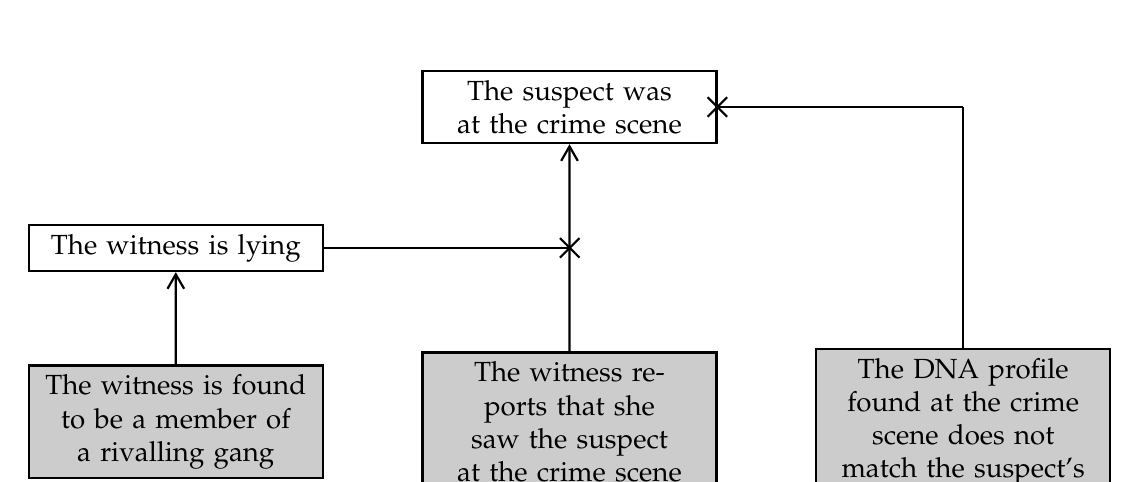
\begin{tikzpicture}[
		scnnode/.append style={text width=3cm},
		arg/.append style={text width=3.5cm},
	]
		\pgftransformxscale{5}
		\pgftransformyscale{2}

		% \draw[thick,dashed,rounded corners=1mm] (-1.45,0.45) rectangle (-0.55,-4.3);
		% \draw[thick,dashed,rounded corners=1mm] (-0.45,0.45) rectangle (0.
		% 45,-4.3);
		% \draw[thick,dashed,rounded corners=1mm] (0.55,0.45) rectangle (1.45,-4.3);

		\node[arg]     (conc) at (-1,0) {The suspect was at the crime scene};
%		\node[arg]     (oppconc) at (0,0) {The suspect was not at the crime scene};
		\node[arg,observed] (prem) at (-1,-2) {The witness reports that she saw the suspect at the crime scene};
		\node[arg,observed] (prem2) at (0,-2) {The DNA profile found at the crime scene does not match the suspect's};
		\node[arg,observed] (prem3) at (-2,-2) {The witness is found to be a member of a rivalling gang};

		\node[arg] (att) at ($(prem.north)!0.5!(conc.south)-(1,0)$) {The witness is lying};

		\draw[arg] (prem3) -- (att);
		\draw[] (prem2) -- (0,0);
		\draw[attack] (0,0) -- (conc);
		\draw[arg] (prem) -- (conc);
%		\draw[arg] (prem2) -- (oppconc);
%		\draw[attack] (prem2) -- (conc);
%		\draw[attack] (conc) -- (oppconc);
%		\draw[attack] (oppconc) -- (conc);
		\draw[attack] (att) -- ($(prem.north)!0.5!(conc.south)$);

	\end{tikzpicture}
\end{document}

\caption{Arguments with supporting and attacking reasons\label{fig:arg}}
\end{figure}

The analysis of the structure of arguments goes back to the early twentieth century when John Henry Wigmore developed his famous evidence charts~\citep{wigmore1913,wigmore1931}. The work by the New Evidence Scholarship~\citep{andersonEtal2005} continued from Wigmore's insights. Independently, and not focusing on evidence in criminal cases, the structure of arguments for and against conclusions was formalized and computationally studied by the philosopher John~\citet{pollock1987,pollock1995}. The work by Pollock stimulated an extensive literature on the formal and computational study of arguments for and against conclusions~\citep{vanEemerenEtal2014Ch11}.

\subsection{Probabilities}
The second normative framework for the correct handling of the evidence uses probabilities as main tool. The probability calculus is used to connect the probabilities of evidence and events, conditioned on each other. Consider for instance a trace found at the crime scene with a rare DNA profile of estimated frequency 1 in a billion. Because the profile is rare, a match is not often found accidentally. This statement can be made precise in the probability calculus. When $E$ expresses the evidence that the suspect's profile matches the trace's and $H$ that the suspect is not the source, we write:

\begin{quotation}
	$\Pr(E|H) = 1/10^9$
\end{quotation}

\noindent Here $\Pr(E|H)$ denotes the conditional probability that the suspect's profile matches the trace's, given the condition that the suspect is not the source. Conditional probabilities obey the famous Bayes' theorem:

\begin{quotation}
	$\Pr(H|E) = \dfrac{\Pr(E|H)}{\Pr(E)}\cdot\Pr(H)$
\end{quotation}

\noindent This formula shows how the posterior probability $\Pr(H|E)$ of the hypothesis given the evidence can be computed by multiplying the prior probability $\Pr(H)$ and the Bayes factor $\Pr(E|H)/\Pr(E)$.

[THE TREATMENT OF BAYES THEOREM IS BRIEF AND IT'S 
UNCLEAR HOW IT IS CONNECTED WITH THE RANDOM MATCH PROBABILITY.]

The interest in probabilistic calculations as a tool for the good handling of the evidence has recently been stimulated by the statistics related to DNA profiling, and by some infamous miscarriages of justice that involved statistics, in particular the Lucia de Berk and Sally Clark cases~\citep{dawidEtal2011,fenton2011,schnepsColmez2013}. The interest is not new~\citep{tillers2011}, and can in fact be traced back to early forensic science in the late nineteenth century~\citep{taroniEtal1998}. To what extent probabilistic calculations have a place in courts has always been, and remains the subject of debate.\footnote{A recent instance of the debate concerns the R v T case, where the UK Court of Appeal restricted the use of Bayes' theorem in courts to cases with a solid statistical foundation such as DNA; see the 2012 special issue of Law, Probability and Risk; Vol. 4, No. 2. For a 1970s instance of the debate, see~\citet{finkelsteinFairley1970,tribe1971}.}

\subsection{Scenarios}
\label{sec:introScen}
The third normative framework for the correct handling of the evidence centers around scenario analysis. In a scenario, a coherent account of what may have happened in a case is made explicit. Different scenarios are contrasted, and evaluated, by considering their plausibility and by checking to what extent they match and contradict the available evidence. 

For instance, consider a murder case with two suspects: the victim's former partner and a robber. For each suspect, a scenario is considered that explains the murder:

\begin{description}
	\item $S_1$: The victim's former partner killed the victim after a fight.
	\item $S_2$: The robber killed the victim when caught during a robbery.	
\end{description}

\noindent When the robber confesses having killed the victim during a robbery, there is evidence contradicting scenario $S_1$ and matching scenario $S_2$.

Scenario analysis proves helpful when considering a complex case and its evidence. The coherent explanation of the evidence provided by a scenario can be regarded as a sense-making tool for handling cases with a large dossier. In particular, legal psychology has contributed to our knowledge about the role of scenarios in handling the evidence~\citep{bennettFeldman1981,penningtonHastie1993}. Scenarios were shown to be misleading, as experiments showed that a false scenario told in a sensible chronological order was more easily believed than a true scenario that was told in a random order. Still, the legal psychologists~\citet{wagenaarEtal1993} emphasised the usefulness of scenario analysis for the rational handling of the evidence, using the technique in their work on debunking dubious case decisions. Scenario analysis is connected with inference to the best explanation~\citep{pardoAllen2008}.

[I THINK WE SHOUD MAKE CLEAR THAT EACH FRAMEWORK WILL BE 
DEVELOPED MORE IN DEPTH LATER IN THE PAPER AND THAT IN THIS FIRST SECTION WE ARE 
BEING GENERAL AND IMPRESSIONISTIC. THIS SECTIONS LOOKS LIKE 
A SUMMARY FO WHAT'S TO COME.]

\subsection{Paper plan}

The three normative frameworks for the handling of evidence, arguments, scenarios, and probabilities, are connected to the first three of the central questions that we have discussed:

\begin{description}
	\item Question 1: How should we handle conflicting evidence?
	\item Question 2: How should we handle the strength of the evidence?
	\item Question 3: How should we coherently interpret the available evidence? 
\end{description}

\noindent Although---as we shall see---each of the three normative frameworks provides relevant insights for answering each of these three questions, the first question about conflicting evidence is especially closely related to the arguments framework, the second question about strength of the evidence in particular to the probabilities framework, and the third question about coherently interpreting the evidence most strongly to the scenarios framework.

[UNSURE ABOUT THIS PART. IT IS PARTLY A REPETITION OF THE QUESTIONS WE ALREADY FORMULATED EARLIER. ALSO, REGARDING THE FACT THAT EACH 
FRAMEWORK IS MORE CLOSELY CONNECTED TO A SPECIFIC TYPE OF QUESTION, THE READER MIGHT NOT CARE TOO MUCH ABOUT IT. WE COULD SAY THAT AT THE END.]

In the following sections, these three questions will be discussed, consecutively, while emphasizing 
the role of the three normative frameworks (Sections~\ref{sec:conf},~\ref{sec:str} and~\ref{sec:cohint}). 
The final question (Section ~\ref{sec:whenconv}) ties together the previous ones 
and concerns the decision to convict or acquit based 
on the evaluation of the evidence:

%The remaining two questions are less strongly connected to the normative frameworks, and are discussed in Sections~\ref{sec:intexc} and~\ref{sec:whenconv}:

\begin{description}
	%\item Question 4: How should we collect, include, exclude evidence?
	\item Question 4: How should we decide about the facts given the evidence? When are we done?
\end{description}


[OVERALL, MY IMPRESSION  IS THAT WE ARE NOT GETTING 
INTO THE HEART OF THE MATTER EARLY ENOUGH.]


\section{Conflicting evidence}
\label{sec:conf}
 	
%\paragraph{Evidential reasoning in the law is a dialectical process involving reasons pro and con different reconstructions of the facts.} 

In many situations, it is clear what the facts are. In a possible case of tax evasion, it will be easy to establish whether you filed for taxes on time and that your employer paid you 100,000 dollars in 2015. Only in special circumstances, such as administrative errors, there will be something to dispute here. 
Cases that are litigated in court are typically more complicated.
Disputes emerge because the two parties---who then become the defense and the 
prosecutor in a criminal trial---introduce evidence that support conflicting 
reconstructions of the facts. 

%For example, a witness for the prosecutor may assert she saw the 
%defendant around the crime scene at the time of the crime, 
%while the defense may introduce evidence that the genetic material found 
%at the crime scene does not match the defendant's.


\subsection{Arguments}
\label{sec:confArg}


In the argumentative normative framework, the handling of conflicting evidence is analyzed in terms of the arguments for and against the different positions considered.

\paragraph{The arguments for and against different positions have structure, involving complexes of reasons supporting and attacking positions.} 

Consider a crime case, where a witness reports that she saw the suspect at the crime scene. Then there is a reason supporting that the suspect indeed was at the crime scene, which in turn provides some support to the conclusion that the suspect committed the crime. This chain of supporting reasons is graphically depicted in Figure~\ref{fig:arg2}, on the left. 
When it is now discovered that the witness is a member of a rivaling gang, there is reason to believe that she is lying (Figure~\ref{fig:arg2}, on the right). The reason that the witness is lying attacks the argument on the left, in the sense that the witness testimony no longer provides support for the suspect being at the crime scene.

\begin{figure}[bt]
\centering
\documentclass[border=5mm,tikz]{standalone} 

\usepackage{amsmath}
% !TEX root=img/arguments_and_attack.tex

% \usetikzlibrary{external} 
% \tikzexternalize[prefix=tikz/] 

\usetikzlibrary{calc}
\usetikzlibrary{arrows}
\usetikzlibrary{arrows.meta}
\usetikzlibrary{decorations.markings}
% \usetikzlibrary{intersections}
\usetikzlibrary{fit}
\usetikzlibrary{shapes}
% \usetikzlibrary{trees}


\tikzset{
	every path/.style={thick},
	align=center,
	observed/.style={
		fill=black!20,
	},
	bn/.style={
		draw,
		ellipse,
		-{Triangle[angle=60:6pt 0]}
	},
	scn/.style={
		draw,
		rectangle,
		% signal,
		% signal from=west,
		% signal pointer angle=120,
		-{Triangle[angle=60:6pt 0]},
	},
	possibly/.style={dashed},
	arg/.style={
		draw,
		rectangle,
		-{Straight Barb[angle=60:6pt 0]}
	},
	attack/.style={
		-{Rays[width=10pt,length=10pt,sep=-3.9pt]}
	},
	pref/.style={
		draw,
		rectangle,
		-{Straight Barb[angle=60:6pt 0]}
	},
	subscn/.style={
		double,
		-{Triangle[angle=60:6pt 0]},
	},
	specific/.style={
		double,
		-{Stealth[angle=60:6pt 0]}
	},
}



\begin{document}
	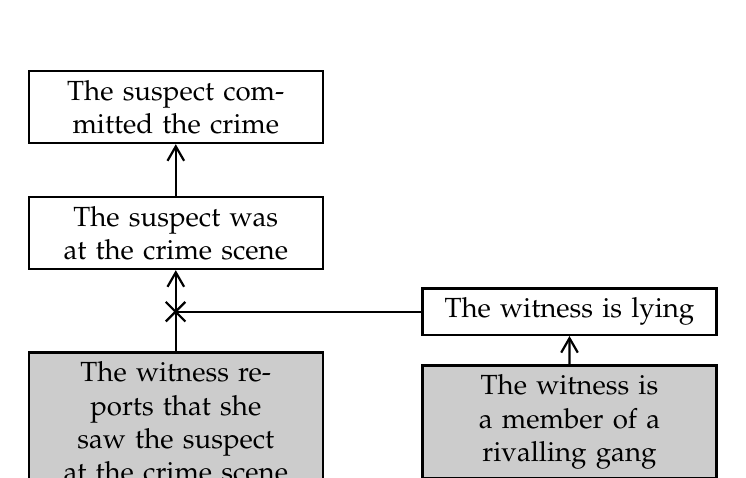
\begin{tikzpicture}[
		scnnode/.append style={text width=3cm},
		arg/.append style={text width=3.5cm},
	]
		\pgftransformxscale{5}
		\pgftransformyscale{2}

		\node[arg]     			(comm) at (0,0) {The suspect committed the crime};
		\node[arg]     			(scene) at (0,-0.8) {The suspect was at the crime scene};
		\node[arg,observed] (witn) at (0,-2) {The witness reports that she saw the suspect at the crime scene};

		\draw[arg] 					(witn) -- (scene);
		\draw[arg] 					(scene) -- (comm);

		\node[arg] 					(lying) at (1,-1.3) {The witness is lying};
		\node[arg,observed] (rival) at (1,-2) {The witness is a member of a rivalling gang};

		\draw[attack] 			(lying) -- (0, -1.3);
		\draw[arg] 					(rival) -- (lying);

	\end{tikzpicture}
\end{document}

\caption{Arguments have structure\label{fig:arg2}}
\end{figure}

\paragraph{Three kinds of support can be distinguished: multiple, subordinated and coordinated support.}

If we consider the argument thet the suspect was at the crime scene because the witness reports that she saw the suspect at the crime scene, each of the three parts of the argument can be supported: the conclusion, the premise and the connection between the premise and the conclusion. For instance, the conclusion can be supported by a second witness testimony. The premise can be supported by the police report that documents the witness testimony. The connection between the premise and the conclusion can be supported by the trustworthiness of the witness report. Additional support of the conclusion is referred to as multiple support. Additional support of the premise is called subordinating support. Additional support of the connection between the premise and the conclusion does not have a standard name, but is closely related to a third named kind of support: coordinated supported. In coordinated support, the support for the conclusion consists of more than one element that in their conjunctive combination provide support for the conclusion. Coordinated support is distinguished from multiple support since in the latter each element of the support for the conclusion provides support by itself. Figure~\ref{fig:support} shows the three named kinds of support. Note that multiple and subordinated support are graphically visualized with an arrow, whereas coordinated support is shown with a line. An arrow would indicate the unnamed kind of support of the connection between premise and conclusion.

\begin{figure}[bt]
\centering
\documentclass[border=5mm,tikz]{standalone} 

\usepackage{amsmath}
% !TEX root=img/arguments_and_attack.tex

% \usetikzlibrary{external} 
% \tikzexternalize[prefix=tikz/] 

\usetikzlibrary{calc}
\usetikzlibrary{arrows}
\usetikzlibrary{arrows.meta}
\usetikzlibrary{decorations.markings}
% \usetikzlibrary{intersections}
\usetikzlibrary{fit}
\usetikzlibrary{shapes}
% \usetikzlibrary{trees}


\tikzset{
	every path/.style={thick},
	align=center,
	observed/.style={
		fill=black!20,
	},
	bn/.style={
		draw,
		ellipse,
		-{Triangle[angle=60:6pt 0]}
	},
	scn/.style={
		draw,
		rectangle,
		% signal,
		% signal from=west,
		% signal pointer angle=120,
		-{Triangle[angle=60:6pt 0]},
	},
	possibly/.style={dashed},
	arg/.style={
		draw,
		rectangle,
		-{Straight Barb[angle=60:6pt 0]}
	},
	attack/.style={
		-{Rays[width=10pt,length=10pt,sep=-3.9pt]}
	},
	pref/.style={
		draw,
		rectangle,
		-{Straight Barb[angle=60:6pt 0]}
	},
	subscn/.style={
		double,
		-{Triangle[angle=60:6pt 0]},
	},
	specific/.style={
		double,
		-{Stealth[angle=60:6pt 0]}
	},
}



\begin{document}
	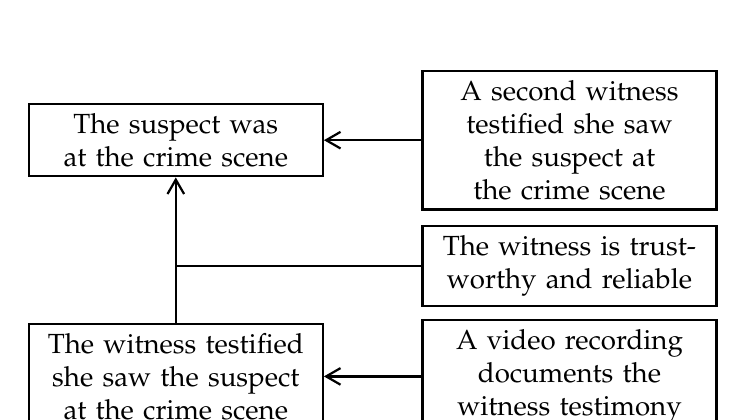
\begin{tikzpicture}[
		scnnode/.append style={text width=3cm},
		arg/.append style={text width=3.5cm},
	]
		\pgftransformxscale{5}
		\pgftransformyscale{2}

		\node[arg]     			(scene) at (0,-0.5) {The suspect was at the crime scene};
		\node[arg] 					(witn) at (0,-2) {The witness testified she saw the suspect at the crime scene};

		\node[arg] 					(alibi) at (1,-0.5) {A second witness testified she saw the suspect at the crime scene};
		\node[arg] 					(lying) at (1,-1.3) {The witness is trustworthy and reliable};
		\node[arg] 					(fraud) at (1,-2) {A video recording documents the witness testimony};

		\draw[arg] 					(witn) -- (scene);

		\draw[arg] 			(alibi) -- (scene);
		\draw 					(lying) -- (0, -1.3);
		\draw[arg] 			(fraud) -- (witn);

%%%

		%\node[arg]     			(scene) at (1.85,-0.5) {The suspect was at the crime scene};
		%\node[arg] 					(witn) at (1.85,-2) {The witness reports that she saw the suspect at the crime scene};
%
		%\node[arg] 					(lying) at (2.35,-1.15) {The witness report is trustworthy};
%
		%\draw[arg] 					(witn) -- (scene);
%
		%\draw 					(lying) -- (1.85, -1.15);




	\end{tikzpicture}
\end{document}

\caption{Three kinds of support\label{fig:support}}
\end{figure}



\paragraph{Three kinds of attack can be distinguished: rebutting, undercutting, and undermining attack.}

Consider again the argument for the position that the suspect was at the crime scene, as supported by the reason of a witness reporting that she saw the suspect at the crime scene (Figure~\ref{fig:arg3}, on the left). This argument can be attacked in three ways. First, its conclusion can be attacked. The suspect can for instance have an alibi, showing that he was not at the crime scene. Such an attacking reason that supports an opposite conclusion is called a rebutting attack. Second, the connection between the reason and the conclusion can be attacked. The lying of the witness is an example of such an attack, referred to as an undercutting attack. In contrast with a rebutting attack, an undercutting attack provides no support for the opposite conclusion. In the example, when the witness is lying, there is no reason supporting that the suspect was not at the crime scene. The attack statement, here the lying of the witness, is also referred to as an exclusionary reason. Third, the reason itself can be attacked. For instance, when the witness report is fraudulent, it can be supported that the witness did not report that she saw the suspect at the crime scene. This kind of attack is referred to as undermining attack. The three examples of the different kinds of attack are shown in Figure~\ref{fig:arg3}, on the right.


\begin{figure}[bt]
\centering
\documentclass[border=5mm,tikz]{standalone} 

\usepackage{amsmath}
% !TEX root=img/arguments_and_attack.tex

% \usetikzlibrary{external} 
% \tikzexternalize[prefix=tikz/] 

\usetikzlibrary{calc}
\usetikzlibrary{arrows}
\usetikzlibrary{arrows.meta}
\usetikzlibrary{decorations.markings}
% \usetikzlibrary{intersections}
\usetikzlibrary{fit}
\usetikzlibrary{shapes}
% \usetikzlibrary{trees}


\tikzset{
	every path/.style={thick},
	align=center,
	observed/.style={
		fill=black!20,
	},
	bn/.style={
		draw,
		ellipse,
		-{Triangle[angle=60:6pt 0]}
	},
	scn/.style={
		draw,
		rectangle,
		% signal,
		% signal from=west,
		% signal pointer angle=120,
		-{Triangle[angle=60:6pt 0]},
	},
	possibly/.style={dashed},
	arg/.style={
		draw,
		rectangle,
		-{Straight Barb[angle=60:6pt 0]}
	},
	attack/.style={
		-{Rays[width=10pt,length=10pt,sep=-3.9pt]}
	},
	pref/.style={
		draw,
		rectangle,
		-{Straight Barb[angle=60:6pt 0]}
	},
	subscn/.style={
		double,
		-{Triangle[angle=60:6pt 0]},
	},
	specific/.style={
		double,
		-{Stealth[angle=60:6pt 0]}
	},
}



\begin{document}
	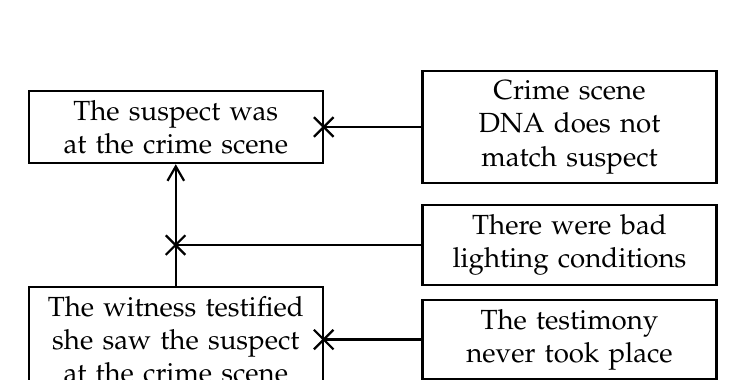
\begin{tikzpicture}[
		scnnode/.append style={text width=3cm},
		arg/.append style={text width=3.5cm},
	]
		\pgftransformxscale{5}
		\pgftransformyscale{2}

		\node[arg]     			(scene) at (0,-0.65) {The suspect was at the crime scene};
		\node[arg] (witn) at (0,-2) {The witness testified she saw the suspect at the crime scene};

		%\node[arg] 					(alibi) at (1,-0.65) {The suspect has an alibi}; 
		\node[arg] 					(alibi) at (1,-0.65) {Crime scene DNA does not match suspect}; 
		%\node[arg] 					(lying) at (1,-1.3) {The witness is lying};
		\node[arg] 					(lying) at (1,-1.4) {There were bad lighting conditions};
		\node[arg] 					(fraud) at (1,-2) {The testimony never took place};

		\draw[arg] 					(witn) -- (scene);

		\draw[attack] 			(alibi) -- (scene);
		\draw[attack] 			(lying) -- (0, -1.4);
		\draw[attack] 			(fraud) -- (witn);

	\end{tikzpicture}
\end{document}

\caption{Three kinds of attack\label{fig:arg3}}
\end{figure}

%\paragraph{In an argumentative dialogue, parties take positions supported by reasons that can be challenged by attacking reasons.}
%
%Arguments have a dialogical counterpart, in which parties exchange reasons for and against the positions they endorse. The arguments shown in Figure~\ref{fig:arg2} for instance form the backbone of the following argumentative dialogue---here presented as a fictitious, stylized discussion between judge, prosecution and defense:
%
%\begin{description}
	%\item \emph{Prosecution}: The suspect committed the crime.
	%\item \emph{Judge}: Why do you believe that?
	%\item \emph{Prosecution}: The suspect was at the crime scene.
	%\item \emph{Judge}: Do you have evidence supporting that position?
	%\item \emph{Prosecution}: There is a witness reporting that she saw the suspect at the crime scene.
	%\item \emph{Defense}: Objection, your honor! The witness is lying.
	%\item \emph{Judge}: Why do you believe that?
	%\item \emph{Defense}: The witness is a member of a rivalling gang.
%\end{description}
%
%
%
%[I LIKE VERY MUCH THE DESCRIPTION OF THE THREE KINDS OF ATTACKS AND THE GRAPHICAL ILLUSTRATION. BUT THIS PART ABOUT THE DIALOGUE IS STRANGE. 
%FIRST, THE DIALOGUE IS UNNATURAL. SECOND, I AM NOT SURE THIS IS ABOUT ARGUMENTS ANYMORE. ARGUMENTS CAN COME IN THE FORM OF A DIALOGUE 
%BUT  NEED NOT BE. PERHAPS WE NEED TO REDEFINE THE ARGUMENT FRAMEWORK AS DIALOGUE/ARGUMENT FRAMEWORK?]
%
%\noindent Models of argumentative dialogue involve specifications of the kinds of moves parties can make, the commitments these moves imply for parties, and the rules that determine the allowed sequences of dialogue moves.

\paragraph{Further readings} 
Argument structure and diagrams~\citep{wigmore1913,wigmore1931,toulmin1958,freeman1991}. Defeasible reasoning and nonmonotonic logic~\citep{pollock1987,gabbayEtal1994}. Rebutting and undercutting attack~\citep{pollock1987,pollock1995}. Undermining attack~\citep{bondarenkoEtal1997}. Formal evaluation of defeasible arguments~\citep{pollock1987,pollock1995,dung1995,prakken2010}. Argumentative dialogue~\citep{toulmin1958,waltonKrabbe1995,prakken1997,hage2000}. Accrual of reasons and weighing~\citep{pollock1995,hage1997,verheij1996diss,prakken2005}. Argument diagramming and evaluation software~\citep{pollock1995,reedRowe2004,kirschnerEtal2003,vanGelder2003,verheij2005,gordonEtal2007}.

\subsection{Scenarios}

In the scenarios normative framework, the handling of conflicting evidence is analyzed by considering different scenarios about what may have happened.

\paragraph{Scenarios are clusters of events, ordered in time and connected by causal relations.} Consider again the murder example with two suspects: the victim's former partner, who killed the victim after a fight ($S_1$), and a robber who killed the victim when caught during a robbery ($S_2$) (used in Section~\ref{sec:introScen}). Scenario $S_1$ can be made explicit as a sequence of four hypothetical consecutive events (Figure~\ref{fig:scens}). First, the victim and his former partner have a relation ($H_1$); then they break up ($H_2$); subsequently, there is a fight ($H_3$); and finally, the victim is killed by his former partner ($H_4$). Scenario $S_2$ can be analyzed as consisting of three events. First, the robber enters the victim's house ($H_5$); then the victim accidentally encounters the robber ($H_6$); and finally, the robber kills the victim ($H_7$). Some of the events in these chronologically ordered scenarios are causally connected. For instance, in the first scenario, the killing is caused by the break up and the fight; and in the second scenario by the accidental encounter.

\begin{figure}[bt]
\centering
\documentclass[border=5mm,tikz]{standalone} 

\usepackage{amsmath}
% !TEX root=img/arguments_and_attack.tex

% \usetikzlibrary{external} 
% \tikzexternalize[prefix=tikz/] 

\usetikzlibrary{calc}
\usetikzlibrary{arrows}
\usetikzlibrary{arrows.meta}
\usetikzlibrary{decorations.markings}
% \usetikzlibrary{intersections}
\usetikzlibrary{fit}
\usetikzlibrary{shapes}
% \usetikzlibrary{trees}


\tikzset{
	every path/.style={thick},
	align=center,
	observed/.style={
		fill=black!20,
	},
	bn/.style={
		draw,
		ellipse,
		-{Triangle[angle=60:6pt 0]}
	},
	scn/.style={
		draw,
		rectangle,
		% signal,
		% signal from=west,
		% signal pointer angle=120,
		-{Triangle[angle=60:6pt 0]},
	},
	possibly/.style={dashed},
	arg/.style={
		draw,
		rectangle,
		-{Straight Barb[angle=60:6pt 0]}
	},
	attack/.style={
		-{Rays[width=10pt,length=10pt,sep=-3.9pt]}
	},
	pref/.style={
		draw,
		rectangle,
		-{Straight Barb[angle=60:6pt 0]}
	},
	subscn/.style={
		double,
		-{Triangle[angle=60:6pt 0]},
	},
	specific/.style={
		double,
		-{Stealth[angle=60:6pt 0]}
	},
}



\begin{document}
	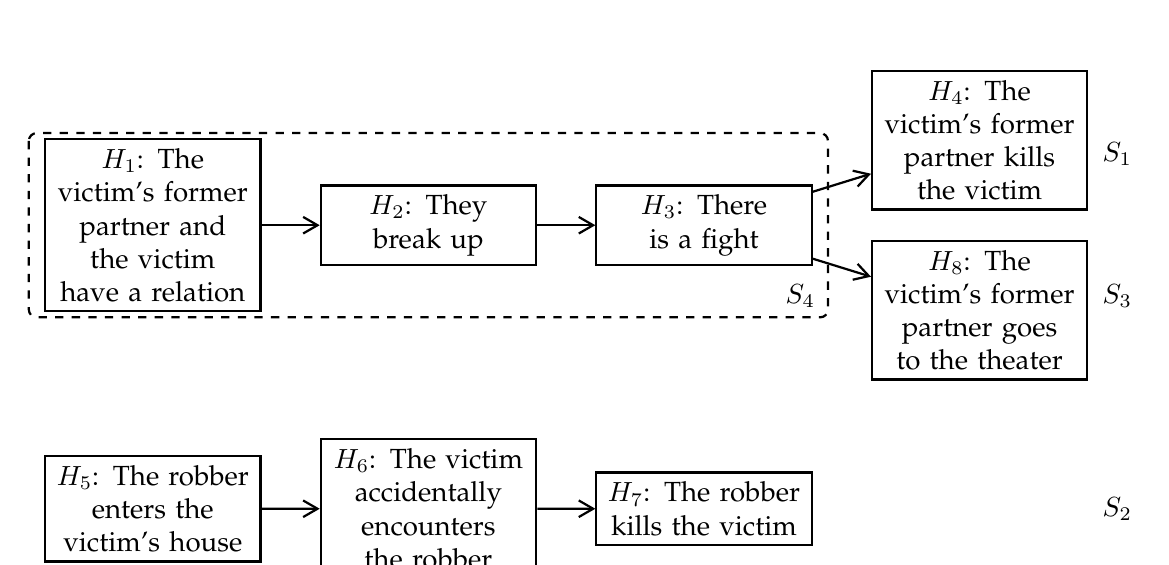
\begin{tikzpicture}[
		scn/.append style={text width=2.5cm},
		arg/.append style={text width=3cm},
	]
		\pgftransformxscale{3.5}
		\pgftransformyscale{1.8}
		
		\node[scn] (H1) at (1,0) {$H_1$: The victim's former partner and the victim have a relation};
		\node[scn] (H2) at (2,0) {$H_2$: They break up};
		\node[scn] (H3) at (3,0) {$H_3$: There is a fight};

		\node[scn] (H4) at (4,0.6) {$H_4$: The victim's former partner kills the victim};

		\node at (4.5,0.5) {$S_1$};

		\node[scn] (H8) at (4,-0.6) {$H_8$: The victim's former partner goes to the theater};

		\node at (4.5,-0.5) {$S_3$};

		\node[scn] (H5) at (1,-2) {$H_5$: The robber enters the victim's house};
		\node[scn] (H6) at (2,-2) {$H_6$: The victim accidentally encounters the robber};
		\node[scn] (H7) at (3,-2) {$H_7$: The robber kills the victim};

		\node at (4.5,-2) {$S_2$};

		\draw[thick,dashed,rounded corners=1mm] (0.55,0.65) rectangle (3.45,-0.65);
		\node at (3.35,-0.5) {$S_4$};

		\draw[arg] (H1) -- (H2);
		\draw[arg] (H2) -- (H3);
		\draw[arg] (H3) -- (H4);
		\draw[arg] (H3) -- (H8);
		\draw[arg] (H5) -- (H6);
		\draw[arg] (H6) -- (H7);


	\end{tikzpicture}
\end{document}

\caption{Alternative scenarios and their structure\label{fig:scens}}
\end{figure}

\paragraph{Scenarios can explain a piece of evidence or be contradicted by it.} The starting point of the murder investigation is the victim's body found at the crime scene (evidence $E_0$). There are two alternative scenarios that explain this evidence: Both the former partner murder scenario $S_1$ and the robbery murder scenario $S_2$ explain evidence $E_0$, in the sense that finding the body is expected assuming the scenario to be true. Assume now that a match is found between the DNA profile of a tissue trace found under the victim's finger nails and that of his former partner (evidence $E_1$). This evidence is explained by scenario $S_1$, but not by $S_2$, of which evidence $E_1$ is independent. 

When the former partner is confronted with the DNA evidence, she provides a different scenario that explains evidence $E_1$: Indeed there was a fight about the break up, but she did not kill the victim, and instead subsequently went to the theater (scenario $S_3$; Figure~\ref{fig:scens}). So we have two scenarios explaining the DNA profile match $E_1$: the former partner murder scenario $S_1$ and the former partner alibi scenario $S_3$. In fact, the two scenarios share a subscenario about the break up fight, that explains the finding of the match (scenario $S_4$ in Figure~\ref{fig:scens}).

When checking the alibi scenario, it is found that the victim's former partner's bank card was used at the theater that night (evidence $E_2$), contradicting the former partner murder scenario $S_1$. Scenario $S_3$ explains both the DNA evidence $E_1$ and the use of the bank card $E_2$. 

\paragraph{Scenarios considered may or may not solve a case, and show which evidence is legally relevant.} A criminal case is only solved when the legally relevant circumstances can be proven. For instance, in murder cases, it should be proven who killed the victim and why. Of the scenarios considered, the former partner murder scenario $S_1$ and the robbery murder scenario $S_2$ explain how and why the murder happened, but the alibi scenario $S_3$ does not. In a crime investigation, it can be hard to find evidence that proves a sufficiently detailed scenario about what has happened. For instance, in the example, it is initially clear that a murder had happened, but not by who. Because of the break up, a scenario that answers the why-question is considered: the former partner murder scenario $S_1$. That scenario is initially corroborated by the DNA match $E_1$, but then breaks down by the use of the bank card $E_2$ that proves the alibi scenario $S_3$. Only when the robber is caught and confesses having killed the victim (evidence $E_3$)---possibly much later, it becomes clear what has happened. The body found $E_0$ and the confession $E_3$ are relevant for answering the legally relevant questions who killed the victim and why. The other evidence considered, the DNA match $E_1$ and the use of the bank card $E_2$, have played a relevant role in the investigation, but do not support or contradict robbery murder scenario $S_2$. 

			%E0			E1			E2			E3
%S1		expl		expl		ind			ind
%S2 		expl		ind			ind			expl
%
%S3		ind			expl		expl		ind
%
%S4		ind			expl		ind			ind
%S2+S3	expl		expl		expl		expl




%\paragraph{Several scenarios and their relations}
%
%In the scenario framework, it is natural to consider several mutually inconsistent scenarios simultaneously. Scenarios can have different relations with one another. They can be mutually inconsistent, such as the two murder scenarios $S_1$ and $S_3$ that each assume a different killer. They can be compatible, such as the innocent former partner scenario $S_2$ and the caught robber scenario $S_3$ that both can be true. They can have subscenario relations, such as the break up fight scenario $S_4$ (in the figure consisting of the events $H_1$, $H_2$ and $H_3$) that is a subscenario of the two scenarios $S_1$ and $S_2$ involving the victim's former partner.
%
%
%\paragraph{Scenarios as alternative explanations of the evidence}
%
%Scenarios can be considered as alternative explanations of the evidence. Returning to the three pieces of evidence discussed in Section~\ref{sec:introScen}, we see that the breakup murder scenario $S1$ explains the skin trace $E1$, the innocent former partner scenario $S2$ explains the skin trace $E1$ and the bank card use $E2$, and the caught robber scenario explains the confession $E3$.
%
%
%
%\textbf{COPIED FROM THAT SECTION; REORGANIZE; my suggestion: that section even briefer.} the breakup murder scenario $S1$ explains the skin trace $E1$, but is contradicted by the use of the bank card $E2$, and again by the confession $E3$. The innocent former partner scenario $S2$ explains the skin trace $E1$ and the bank card use $E2$, and is independent from the confession $E3$. The caught robber scenario explains the confession $E3$, and is independent from the skin trace $E1$ and the bank card use $E2$. Considering these scenarios and this evidence, breakup murder scenario $S1$ is hard to believe, the innocent former partner and caught robber scenarios $S2$ and $S3$ seem to be true.
%
%\paragraph{Comparative adequacy of alternative scenarios/hypotheses in explaining the evidence}
%


[THIS SECTION IS VERY INTERESTED, BUT PERHAPS TOO SOPHISTICATED. 
I WONDER IF IT CAN BE MADE SIMPLER. IT SEEMS TO ME THAT THE ARGUMENT SECTION WAS SIMPLY ABOUT HOW ARGUMENTS CAN CONFLICT, 
BUT THIS SECTION DOES MORE WITH SCENARIOS. IT SHOWS NOT ONLY HOW SCENARIOS CAN CONFLICT BUT ALSO HOW THEY CAN BE COMPARED. 
IT  SHOWS WHICH SCENARIO IS THE BEST AND ADDRESSES -- TO A CERTAIN EXTENT, AT LEAST -- THE QUESTION HOW CASES CAN BE SOLVED. 
THIS BELONGS TO LATER IN THE CHAPTER. ]


\paragraph{Further readings} 

\cite{bennettFeldman1981,penningtonHastie1993,penningtonHastie1993StoryModel,wagenaarEtal1993}

\subsection{Probabilities}

In the probabilistic normative framework, the handling of conflicting evidence is analyzed in terms of the conditional probabilities that connect the evidence and the hypotheses.

\paragraph{Evidential favoring and disfavoring can be characterized as ``probability relevance''} 
%BV:I changed difference to relevance, as 'prob diff' is used later for something else.
%BV:I prefer replacing 'favoring and disfavoring' by 'suport ad attack', throughout.
A piece of evidence $E$ favors an 
hypothesis $H$ whenever $E$ raises the probability of $H$, or in symbols, 
$P(H|E) > P(H)$. 
For example, a witness 
testifies that she saw the defendant around the crime scene
 at the time of the crime. The testimony favors the hypothesis 
 that the defendant is guilty. 
This can be described probabilistically, as follows:
 %
 \[ P(\textit{guilt}|\textit{testimony}) > P(\textit{guilt}).\] 
 %
By contrast, a piece of evidence $E$ disfavors an hypothesis $H$ whenever $E$ lowers 
the probability of $H$, or in symbols, $P(H|E) < P(H)$.
For example, if a DNA test shows no match between the traces found at the crime
 scene and the defendant, this evidence disfavors the hypothesis that the defendant is guilty. 
 Probabilistically, 
%
\[ P(\textit{guilt}|\textit{no DNA match}) < P(\textit{guilt}).\]  
%
 %
 
% \paragraph{Two characterizations of evidential favoring and disfavoring are equivalent} 
\paragraph{Evidential favoring and disfavoring can be characterized as ``likelihood ratio''} 

There is another characterization of evidential favoring and disfavoring. 
Instead of comparing the initial probability $P(H)$ and the probability $P(H|E)$ 
of the hypothesis given the evidence, a so-called likelihood ratio of 
the form ${P(E| H)}/{P(E |\neg H)}$ 
%BV: I changed the vertical fraction to a horizontal one. Looks better inline. I prefer that everywhere.
can also be used.
On this account, $E$ favors $H$ whenever the likelihood ratio
$\frac{P(E|H)}{P(E | \neg H)}$ is greater than one. Intuitively, this means that the presence of the 
evidence is more probable %BV was 'likely'
if the hypothesis is true than if the hypothesis is false. 
By contrast, a piece of evidence $E$ disfavors an hypothesis $H$ whenever 
the likelihood ratio is lower than one. This means that the presence of the evidence is less likely %BV was 'likely'
if the 
hypothesis is true than if the hypothesis is false. For the two examples considered earlier, we have:
%
 \[\frac{P(\textit{testimony}|\textit{guilt})}{P(\textit{testimony}|\neg \textit{guilt})} > 1, \text{ and }\]
 %
 \[\frac{P(\textit{no DNA match}|\textit{guilt})}{P(\textit{no DNA match}|\neg \textit{guilt})} < 1.\]
%
These two characterizations of evidential favoring/disfavoring---in terms of probability 
increase/decrease, and in terms of a likelihood ratio greater/lower than one---are 
in fact equivalent. 
For the following statements hold:
%
%\[\textit{\text{$E$ favors (or supports) $H$} iff }   P(H|E)> P(H) \textit{ iff }\frac{P(E|H)}{P(E|\neg H)}>1.\]
\[ P(H|E)> P(H) \text{ iff }\frac{P(E|H)}{P(E|\neg H)}>1.\footnote{To see why, recall that 
%
\[ \frac{P(H|E)}{P(\neg H | E)} = \frac{P(E | H)}{P(E| \neg H)}\times \frac{P(H)}{P(\neg H)},\]
%
%BV The LR formula should be in the main text somewhere
%BV I like having this proof. (Source?)
%BV I don't like a long, complex footnote. Let's discuss.
which implies
%
\[\frac{P(E|H)}{P(E|\neg H)}>1 \text{ iff } \frac{P(H|E)}{P(\neg H | E)} > \frac{P(H)}{P(\neg H)}.\]
%
For one direction, if $P(H|E)> P(H)$, then $1- P(H|E)< 1- P(H)$. This means that 
$\frac{P(H|E)}{1- P(H | E)} > \frac{P(H)}{1- P(H)}$, and thus
$\frac{P(H|E)}{P(\neg H | E)} > \frac{P(H)}{P(\neg H)}$. So, by the equivalence above, $\frac{P(E|H)}{P(E|\neg H)}>1$.
For the other direction, if $\frac{P(E|H)}{P(E|\neg H)}>1$, then $\frac{P(H|E)}{P(\neg H | E)} > \frac{P(H)}{P(\neg H)}$, again 
by the equivalence above. 
The latter is the same as $\frac{P(H|E)}{1- P(H | E)} > \frac{P(H)}{1- P(H)}$. To establish $P(H|E)> P(H)$, suppose for contradiction that
$P(H|E) \leq P(H)$, which implies $1- P(H|E) \geq 1- P(H)$. This means that $\frac{P(H|E)}{1- P(H | E)} \leq \frac{P(H)}{1- P(H)}$. 
This contradicts $\frac{P(H|E)}{1- P(H | E)} > \frac{P(H)}{1- P(H)}$, and thus $P(H|E)> P(H)$.}\]
 %
\[ P(H|E) < P(H) \text{ iff}  \frac{P(E|H)}{P(E|\neg H)} < 1.\]
%

\paragraph{The conflict between two pieces of evidence can be described probabilistically}
Two pieces of evidence come into 
conflict with one another insofar as one favors an hypothesis 
and the other disfavors the same hypothesis. 
The conflict can be described probabilistically, in that one piece of evidence increases 
the probability of the hypothesis, while the other decreases it, or equivalently, the likelihood ratio is positive (for one piece 
of evidence) and negative (for the other). 
For example, the testimony that the defendant was around the crime scene conflicts 
with the lack of a DNA match. Probabilistically, the testimony 
increases the probability of the defendant's guilt (or equivalently, the likelihood ratio is greater than one),
while the lack of a DNA match decreases the probability of the same hypothesis 
(or equivalently, the likelihood ratio is lower than one).
%BV Nothing is said about conflict resolution. 

\paragraph{Further readings} 
.........................................................................................

\section{Evidential value}
\label{sec:str}

The evidence found in a criminal investigation has different levels of evidential value: some evidence is very strong, other not so much. How is evidential value handled in each of the three normative frameworks? That is the topic of this section.

\subsection{Probability}



\paragraph{Evidential value can be quantified as probability difference, likelihood ratio or overall probability}
%BV Some reshaping is needed in this section, I'd say. 1. There is the evidential value of a piece of evidence; measured by probabilistic difference or LR (`incremental evidential value'). 2. There is the evidential value of all the evidence, in its totality; measured by the overall conditional prob (`total evidential value'). 3. DNA evidence is a good example, but there are complications.
%BV Below the discussion of the drunk witness is (for me) a complicated way of saying that a drunk witness has (by itself) hardly incremental evidential value. What is the lesson to be taught?
%BV In the part on DNA evidence I'd also reshape. For me the RMP connects a match (an actual match, M) probabilistically with the suspect being the source (S); we did that in the project paper verheijEtal2016. I'd first like to see that discussed, and then explained that there also are complications. Here the so-called hierarchy of propositions should be mentioned. cookEtAl1998, evettEtal2000 if I am correct.
The value of the evidence for, or against, an hypothesis 
can be quantified probabilistically in various ways. 
%The probabilistic framework allows us to quantify the strength of the evidential favoring or support relation between evidence and hypothesis. 
%The are different approaches in the literature. % (FITELSON REFERENCE HERE). 
%Let us begin with quantifying the value of the evidence \textit{for} an hypothesis. 
One approach considers the difference between the probability of 
the hypothesis with and without the evidence, that is, $P(H | E) - P(H)$.
%If $P(H | E)$ is higher than $P(H)$, this means that the evidence lends some support to
%the hypothesis. 
The larger the positive difference, the higher the value of the evidence 
for the hypothesis. 
%By contrast, the larger the negative difference, the higher the value of the evidence against the hypothesis. 
An alternative approach is given by the likelihood ratio $\frac{P(E|H)}{P(E| \neg H)}$. 
%For the evidence to offer some support to the hypothesis, the likelihood ratio should be at least greater than one. 
For any value greater than one, the higher the likelihood ratio, 
the higher the value of the evidence for the hypothesis. %For simplicity, we shall speak of evidential strength 
%in terms of likelihood ratios, as follows:
%
%\begin{quote}
%\textsc{Evidential strength:} The evidential strength of $E$ relative to $H$ is proportional to 
%the likelihood ratio $\frac{P(H|E)}{P(H|\neg E)}$. 
%\end{quote}
%
%By contrast, for any value lower than one, the lower the likelihood ratio 
%the higher value of the evidence against the hypothesis. 
\begin{comment} 
The following table %, whose calculations are approximations based on Bayes' theorem, offers 
offers some illustrations:

\vspace{2mm}
\hspace{0.5cm}
\begin{centering}
\begin{tabular}{lccccc}
\hline
$P(H)$ & Likelihood Ratio & $P(H | E)$ &  $P(H|E)-P(H)$ \\
\hline
0.0001 & 1,000 & 0.09 &  0.0899   \\
%0.001 & 1,000 & 0.049 & 0.5  \\
%0.01  & 1,000 & 0.08  & 0.9 \\
0.1 & 1,000  & 0.99 &  0.89 \\
\hline
%0.5 & 1,000 &   0.999 \\
%0.9 & 1,000 &   0.9999 \\
0.0001 & 10  & 0.001 &  0.0009 \\
0.01 & 10  & 0.09 &  0.08  \\
\hline
\end{tabular}
\end{centering}
\vspace{2mm}

\noindent
%Note that even if the likelihood ratio is high, the probability $P(G|E)$ can 
%still be low if the initial probability $P(H)$ is itself low. 
All in all, a positive difference $P(H|E) - P(H)$ and a likelihood ratio $\frac{P(E|H)}{P(E| \neg H)}$ greater than one
%tell us how much a piece of evidence $E$ can impact upwards the initial 
%probability of a hypothesis $H$. They 
quantify, albeit in different ways, the value of the evidence \textit{for} 
an hypothesis. 
\end{comment}
 By contrast, a negative difference $P(H | E) - P(H)$ and a likelihood ratio lower than one  
quantify the value of the evidence \textit{against} an hypothesis.
The larger the negative difference and the lower the likelihood ratio (for any value below one), 
the higher the value of the evidence against the hypothesis.

%As one can see from the table, there are quantitive 
%differences between the two approaches, but these should 
%not concern us here. Since the most widely used approach to quantify evidential value relies on 
%likelihood ratios, we shall use that, making occasional 
%references to the other approach if necessary. 

%\paragraph{The overall probability is not the same as probability difference and likelihood ratio}

Intuitively, the value of a piece of evidence for or against an hypothesis can also be quantified by the probability 
of the hypothesis given the evidence. The higher, or lower, the probability $P(H|E)$, the higher 
the value of the evidence for, or against, the hypothesis. The probability $P(H|E)$, however, should not be confused with the probability difference or the likelihood ratio. To illustrate, suppose a witness testifies that the defendant beat the victim to death, but as it turns out, the witness 
was drunk at the time, so the evidential value of the testimony in favor of guilt is low. 
If the testimony by the drunk witness is the only incriminating evidence, the probability 
$P(\textit{guilt} | \textit{drunk witness})$ should also be low. Now, it follows that $P(\textit{innocence} | \textit{drunk witness})$ 
should be high insofar as \textit{innocence} is the negation of \textit{guilt}. 
But this seems problematic. A drunk witness, in fact, is of little help in establishing 
innocence (just as it is of little help in establishing guilt).

It is instructive to quantify the value of the testimony in favor of guilt by means of 
the probability difference and the likelihood ratio. Since the witness was drunk, the value of the evidence in favor of guilt is 
low, that is:
%
\[\text{the positive difference $P(\textit{guilt} | \textit{drunk witness}) - P(\textit{guilt})$ is small, and}\]
%
%
\[\text{the likelihood ratio $\frac{P(\textit{guilt} | \textit{drunk witness})}{P(\textit{guilt} | \neg\textit{drunk witness})}$ is only slightly above one}.\] 
%
Similarly, the value of the evidence in favor of innocence is also low, that is:
%
\[\text{the negative difference $P(\textit{innocence} | \textit{drunk witness}) - P(\textit{guilt})$ is small, and}\]
%
%
\[\text{the likelihood ratio $\frac{P(\textit{innocence} | \textit{drunk witness})}{P(\textit{innocence} | \neg\textit{drunk witness})}$ is only slightly below one}.\] 
%
So, the value of the testimony in favor of guilt, and innocence, is low 
in both cases. This means that $P(\textit{guilt} | \textit{drunk witness})$
and $P(\textit{guilt})$ are roughly the same value, and so are $P(\textit{innocence} | \textit{drunk witness})$ 
and $P(\textit{innocence})$. Consequently, if $P(\textit{innocence})$ is high, 
and thus $P(\textit{guilt})$ low, $P(\textit{innocence} | \textit{drunk witness})$ will 
be high, and thus $P(\textit{guilt} | \textit{drunk witness})$ low. %, given the little evidential value of the testimony. 
We should thus not be surprised that $P(\textit{innocence} | \textit{drunk witness})$ is high. 
This is because, by Bayes' theorem, $P(H|E)$ depends on $P(H)$.  
Even if $E$ does not change significantly the probability of $H$, or the likelihood ratio (positive or negative) 
$\frac{P(E|H)}{P(E| \neg H)}$ is small, $P(H|E)$ could still be high or low, insofar as $P(H)$ itself is high or low. 
All in all, we should be careful in not confusing a high probability $P(H|E)$ with a high 
evidential value in terms of a large probability difference or a high likelihood ratio.


\paragraph{Likelihood ratio can quantify the value of DNA evidence}



A widely used measure of evidential value 
is the likelihood ratio. As an illustration, let us determine the likelihood ratio 
of a DNA match in favor of guilt. %, where the match is between
%the crime scene's genetic profile and the defendant's. 
%Suppose the DNA test reports a match between the crime traces and the defendant.  %Given our simplifying assumptions, 
When introduced in court, a DNA match comes with an 
estimated Random Match Probability (RMP).  As explained earlier, this
is the probability that a random person, who 
had nothing to do with the crime, would match. The RMP can also be viewed 
as the estimated frequency of the DNA profile across a sample population. 
%We should bear in mind that genetic profiles are not unique. 
%Based on statistical and genetic modeling,  a profile is expected to occur 
%with a  certainfrequency in a select population. 
%
Now, with some simplifications (on these later), 
the evidential value of the DNA 
match in favor of guilt, in terms of a likelihood ratio, 
is as follows % \citep{Dawid02, Balding2005Weight}:
%
\[
\frac{P(M | G)}{P(M | \neg G)} =   \frac{1}{RMP}.
\]
%
%BV RMP is as yet undefined
The numerator $P(M | G)$ equal 1 because %of our simplifying assumption that 'source' and guilt' are interchangeable 
%and the laboratory test is infallible. If 
if the defendant is guilty%and thus the source of the crime traces
, the lab test will report a match. As for the denominator, 
%keep in mind that $RMP$ is the probability that a random person, 
%unrelated to the crime or the defendant, would be found to have a matching DNA. 
putting $P(M | \neg G)=RMP$ is plausible because the probability that a match would be reported assuming that the defendant was \textit{not} 
the source is roughly the same as the chance that a random person---someone who had no contact with the victim---would match anyway. 
%and because (2) 'source' and 'guilt' are, by assumption, equivalent.
For example, if the RMP is 1 in 200 million, the likelihood ratio would be
%
\[\frac{P(M |G)}{P( M | \neg G)}=\frac{1}{\frac{1}{\text{200 million}}}=\text{200 million}.\]
%
Since the likelihood ratio in question is a high number, the DNA match in favor of guilt 
has a high evidential value. More generally,  the lower the RMP, the higher the evidential value of the match. This is because 
the lower the RMP, the less likely a random person would match. 

It is, however, important to keep track of the simplifying assumptions that were made. 
To see what they were, note that the hypothesis of guilt is not equivalent to 
other propositions, such as the following: %which are progressively more removed from guilt: 

- the \textit{lab reports} that the defendant's 
genetic profile matches with the crime traces;

- the defendant's genetic profile \textit{truly matches} with the crime traces; 

- the defendant is the \textit{source} of the traces; and

%the defendant \textit{left} the crime traces; 

%the defendant \textit{visited} the crime scene; 

%the defendant \textit{participated} in the crime; 

- the defendant is \textit{guilty}.

\noindent
The inference from `reported match'  
to `guilt', passing though the intermediate steps `true match' and 'source', is a complex one, 
and many sources of error may undermine the inference along the way.  
Above we have made three simplifying 
assumptions. 

First, we assumed that the inference from `reported match' to `true match' was unobjectionable, or in other words, we assumed
the DNA test reporting a match (or a non-match) was infallible. This, of course, need be the case because laboratories make mistakes.
A more sophisticated probabilistic analysis will show that a RMP as low as 1/1 billion----which in our simplistic analysis would give rise to a likelihood ratio as high as 1 billion---  
reduces to about 100 likelihood ratio if the  laboratory error rate is 1\%.


Second, consider the inference from `true match' to `source'.
There are many ways this inference can go wrong. Even if one is a true match, one need not be the source. A genetically identical twin or someone else 
who just so happens to have an identical DNA could be the source. It could also be that synthetic genetic material, perfectly matching one's DNA, was planted. 
So, the second simplifying 
assumption we made was that the inference from `true match' to `source' can be undermined by 
one source of error only, namely the possibility that another random individual 
could coincidentally match. This possibility of error is captured by the 
Random Match Probability. 
%If RMP equal 1 in 200, we would expected 1 such profile every two hundred people or the RMP equals 0.5\%. 
Other sources of error---such as, a twin brother or an artificially synthesized DNA could be the source---were disregard. 

The third assumption we made was that whoever is the source of the crime traces must be the perpetrator, 
so `guilt' and `source' were treated as equivalent.  This, of course, need not be the case. One could be the source of the traces without participating in the crime because, for example, 
 one visited the crime scene before or after  the crime took place. Relaxing the identification of the two hypothesis 
further weakens the value of a DNA match in favor of guilt.

From a probabilistic point of view, laboratory errors can be quantified if the lab error rates are available, 
but other sources of error are more difficult to quantify. How often does it happen that 
fake matching DNA is implanted? Or what is the probability of error 
in the inference from `source' to `guilt'?
The moral is that, in weighting the value of DNA match with a high likelihood ratio, 
one should always be wary of the sources of error that were, and were not, taken into account. 
Even if the RMP is very low, this does not mean 
that the evidential value of the DNA match in favor of guilt must be very high. 


\paragraph{Further readings} Introductions to using probability for weighing evidence 
 \citep{finkelsteinFairley1970, dawid2002, mortera2007}. Critique 
of the probabilistic approach \citep{tribe1971, cohen1977, allenPardo2007}.
Prosecutor's fallacy \citep{thompsonSchuman1987}.
Introduction to DNA evidence \citep{wasserman2008, kayeSensabaugh2000}.
Different hypotheses for evaluating DNA evidence \citep{koehler1993, cookEtAl1998, evettEtal2000}. 
Probabilistic analyses of DNA evidence  \citep{robertsonVignaux1995, buckleton2005, balding2005}. 
 Lab errors for DNA evidence \citep{thompsonEtAl2003}. 
 Match is not all-or-nothing judgment \citep{kaye1993}. 
Uniqueness of DNA profiles  \citep{kaye2013, weir2007}.
How DNA evidence can be synthesized and implanted \citep{frumkinEtAl2009}. 
Cold hit controversy in DNA evidence cases \citep{NRC1996, baldingDonnely1996}. 
Comparison between DNA evidence and fingerprints  \citep{zabell2005}. 
Probabilistic analyses of eyewitness testimony \citep{friedman1987, schumStarace2001}. 

\subsection{Arguments}
\label{sec:valueArgs}

The evidential value of arguments can be analyzed in terms of the reasons they are built from.

\paragraph{The reasons used in arguments have different strengths. Some are conclusive, others defeasible.} A reason is conclusive when, given  the reason, its conclusion is guaranteed. The main type of conclusive reasons correspond to deductive, logically valid arguments. [WHAT DOES IT MEAN THAT A REASON CORRESPONDS TO AN ARGUMENT?] An example of a conclusive reason occurs in the logically valid argument from the reason `The witness saw the suspect commit the crime and the suspect denies having been at the crime scene' to the conclusion `The suspect denies having been at the crime scene'. Its logical validity is connected to the underlying logical structure of the argument: From A AND B, conclude B. 

[IT IS ODD TO READ 'REASON' WHILE WHAT IT MEANS IS 'PREMISE'. SEEMS STANDARD TO TALK ABOUT PREMISES AND CONCLUSIONS, WHILE YOU SEEM TO PREFER CONCLUSIONS 
AND REASONS. IS THERE SOMETHING SPECIFIC ABOUT THIS? MAYBE SAY SOMEWHERE WE WIL USE 'REASON' TO MEAN 'PREMISE'?]

Many reasons are not conclusive, but defeasible: There are circumstances in which the conclusion does not follow, although the reason obtains. The reason `The witness reports to have seen the suspect at the crime scene' supports the conclusion `The suspect was at the crime scene', but does not guarantee that conclusion, as---for instance---the witness can have been lying or have made a mistake. A defeasible reason can provide prima facie justification for a conclusion, that is withdrawn in light of further information.

[IT IS STRANGE TO READ THAT A REASON IS DEFEASIBLE OR CONCLUSIVE. AN ARGUMENT IS, NOT THE REASON ITSELF. IT DEPENDS WHAT IT IS A REAOSN OF. CONFUSED ABOUT THIS.]

Conclusive and defeasible reasons correspond to one-step conclusive and defeasible arguments. [AGAIN, UNCLEAR TO ME IN WHAT SENSE A REASONS CORRESPONDS 
TO AN ARGUMENT. I THOUGHT REASON CORRESPONDED TO PREMISE.] Some other terms are used in connection with the difference between conclusive and defeasible arguments. For instance, there is the triplet of deductive, abductive, and inductive arguments. Consider the rule `If someone is shot, he dies'. A deductive argument involving this rule applies the rule to an instance of its antecedent: From `John is shot' and `If someone is shot, he dies', conclude `John dies'. An abductive argument using this rule uses an instance of the rule's consequent as a starting point, to infer the antecedent: From `John dies' and  `If someone is shot, he dies', conclude `John is shot'. Abductive arguments can be thought of as providing an explanation. Abductive arguments are typically defeasible, since there often are alternative explanations. Inductive arguments generalize from an instance of the rule's antecedent and consequent (or several such instances) to the rule: From `John is shot' and `John dies', conclude: `If someone is shot, he dies'. Inductive arguments are also typically defeasible, as the inferred rule often does not hold, at least not in full generality. Deductive arguments are also contrasted with ampliative arguments. In that distinction, deductive arguments only lead to conclusions that were already implicit in their premises, whereas ampliative arguments go beyong their premises. Arguing from A AND B to B is deductive in this sense, and from A to B ampliative.

[NOT SURE WE NEED ALL THIS TERMINOLOGY. COMPLICATED. REALLY NEEDED?]


\paragraph{The reasons in arguments can be tested using critical questions.} Defeasible reasons are characterized by the possibility of circumstances that have the effect that the conclusion of the reason does not follow, given the reason. 
[YOU TALK ABOUT CONCLUSION OF THE REASON. LOOKS LIKE YOU ARE USING 'REASON' AS THE SAME AS 'ARGUMENT'. ISN'T THIS STRANGE?]
The occurrence of such defeating circumstances can be guided by asking critical questions. The answers to those critical questions provide insight into the evidential value of the reasons. Consider for instance one-step argument from the reason `The witness reports that she saw the suspect at the crime' to the conclusion `The suspect was at the crime scene'. [NOW YOU USE 'REASON' AS THE SAME AS 'PREMISE'.] 
Critical questions that can be asked include `Are there reasons showing that the suspect was not at the crime scene, such as an alibi?', `Was the witness lying?' and `Are there reasons to think that the witness report is fraudulent?'. The first of these questions is directed at the argument's conclusion, the second at the argument step, and the third at the argument's reason. These different kinds of critical questions are connected to the kinds of argument attack discussed in Section~\ref{sec:confArg} (see in particular Figure~\ref{fig:arg3}).

\paragraph{Further readings} 
deductive, inductive, abductive
deductive, ampliative

Mention ?Pollock's anti-probabilism

Argument scheme collections

Accrual

Reason-Based Logic

\begin{comment}


\paragraph{Args win when they can defend themselves against attacks (Dung 1995)}

Dung REFERENCE provided an abstract framework to analyze 
systems of arguments. The notion of an argument attacking another argument 
is taken as primitive. We can think of systems of argument as an alliance of arguments, and in particular, 
following Dung's framework, the system $S$ of arguments is a \textit{successful alliance} provided:
%
\begin{quote}
(\textit{conflict-free}) each argument in $S$ is not attacked by any argument in $S$; and 

(\textit{defense}) for any argument (outside $S$) that attacks any argument in $S$, there is an argument inside $S$ that attacks the attacker.
\end{quote}
%
So, a system of arguments forms a successful alliance provided there is no internal conflict and any external attack 
can be counterattacked by arguments within the alliance. The notions of a winning and losing argument can now be defined:
%
\begin{quote}
(\textit{winning})  $A$ \textit{wins} provided $A$ is part of a successful alliance; and 

(\textit{losing} ) $A$ \textit{loses} provided another argument $A'$ attacks $A$ and $A'$ wins. 
\end{quote}
%
These definitions are intuitive. If an argument can defend itself from any attack by appealing to its allies, it wins. If, instead, there is a winning argument that attacks an argument, the latter loses. A problem here, however, is that an argument can be both winning and losing. 
Consider four arguments $A, B$ and $A', B'$ such that $A'$ attacks $A$ and vice versa, and $B$ attacks $B'$ and vice versa. The system $\{A, B\}$ is a successful alliance because there are no internal conflicts and any attack against $A$ or $B$ is counterattacked within the alliance $\{A, B\}$. It follows that arguments $A$ and $B$  both win. At the same time, the system $\{ A', B'\}$ is also 
a successful alliance, so arguments $A'$ and $B'$ win. This means that $A$ and $B$ both lose because each is attacked by a winning argument, and the same holds for $A'$ and $B'$.

%(Intuitively, alliance $\{A, B\}$ and $\{A', B'\}$ are symmetrical in the sense that any argument in one alliance is attacked but an argument in the other alliance. No one appears to be stronger then the other. If, however, we compared $\{A, B, C\}$ and $\{A', B'\}$ and added the condition that $C$ attacks either $A'$ or $B'$ and $\{A, B, C\}$ had no internal conflicts, it would follow that $\{A', B'\}$ is not a successful alliance anymore and thus the only winning arguments would be $A$ and $B$. One easy fix could be to require that successful alliances cannot be symmetrical to other successful alliance. This means for any give set of arguments there is only one successful alliances.)

(As far as evidential reasoning in the law is concerned, something is unsettling about this state of affairs. There is something unnatural about the systems $\{A, B\}$ and $\{A', B'\}$ and the fact that $A$ attack $A'$ and vice versa, and the same holds for $B$ and $B'$.
Suppose an eyewitness asserts she saw the defendant stab the victim and another witness asserts the eyewitness is biased because she has reasons to hate the defendant. The second witness attacks the testimony of the eyewitness. This exemplifies an attack against $A$ by $A'$. There is nothing problematic about that. But now suppose the eyewitness defended herself against the second witness by asserting that the second witness is biased against her because the witness has reasons to hate her. This exemplifies a situation in which $A$ attacks $A'$. There is nothing problematic about that either. But, although the fact that $A$ attacks $A'$ and vice versa are fine as isolated attacks, when they are considered together, they become  problematic. Suppose we engage in a conversation in which I assert conclusion $C$ on the basis of evidence $e$  and you challenge me by challenging $e$ on the basis of other evidence $e'$. Next, I defend myself by challenging your evidence $e'$ and I do so by using my evidence $e$.  You challenge targets $e$ on the basis of $e'$ and I target $e'$ on the basis of $e$. This is a stale mate and a circle of attack and counterattack. Ideally, we would need further evidence, besides $e$ and $e'$, to resolve the controversy. In the court example,  a third witness is needed who can tell us whether the first eyewitness or the second witness is biased. So, an easy fix to the above problem, especially when it comes to evidential reasoning in the law, is to require that stalemate situations or circles of attacks and counterattacks be avoided.)

\paragraph{Args win when they are better/stronger than/preferred over conflicting args}

Dung's framework considers system of arguments and the relations of attack and counterattack among arguments, but does not examine the internal structure of arguments. The notions of attack and counterattack are left unspecified, and the notion of a successful 
attack is also left unspecified. To be sure, all we can say from Dung's framework is that an attack is successful when 
it consists of a winning argument. We are told nothing more about the internal structure of arguments.

 Prakken REFERENCE has provided a unified theory of argumentation which builds on Dung's insights but also examines 
 the internal structure of arguments. As seen earlier, argument can be attacked in three ways. An argument can be attacked by offering another argument with the opposite conclusion (rebutting). An argument can be attacked by offering an argument that weakens the inferential link between premises and conclusion (undercutting). An argument can be attacked by challenging its premises (undermining). The remaining question is, when is an attack successful? 

Let us begin with an example of one argument rebutting another.  A witness asserts that the defendant stabbed the victim, while DNA evidence shows no match between the defendant and the crime traces. The argument based on an witness statements is rebutted by---but also rebuts---the argument based on the DNA match. The attack works in both direction in the sense that bother arguments attack one another regardless of which argument is made first. Is the attack successful? In Dung's framework, the answer is that both arguments win and both arguments lose (provided both arguments are part of a successful alliance). This is hardly satisfying. 

A step forward is a ranking among arguments. A rebutting argument $A'$ is considered a successful attack  on an argument $A$ whenver $A$ is ranked higher than $A'$.  How can arguments be ranked? The ranking will depend on the relative strength we assign to the premises and to the inferential link between premises and conclusion. Consider an abstract example. The first argument consists of premises $A$ and the defeasible inference $A\Rightarrow B$, while the second argument consists of premises $A'$ and the defeasible inference $A'\Rightarrow \neg B$. The conclusion of the first argument is $B$ and the conclusion of the second argument is the negation of $B$. Which argument ranks higher? This will depend on whether we consider $A$ a better premise---for example, more probable---than $A'$. It will also depend on whether we consider $A\Rightarrow B$ a better inference---for example, more likely to preserve the truth---than $A'\Rightarrow \neg B$. Clearly, other things being equal, if $A$ is better than $A'$, the first argument is ranked higher. However, if $A$ is a better premise but $A'\Rightarrow \neg B$ is a better inference, it is not easy to adjudicate the ranking of the two arguments.

Consider now a case in which an argument undercuts another argument. There is nothing peculiar about this case. We can apply the same ideas as in the rebutting case. In order for the attack to be successful, the undercutting argument must be ranked higher than the attacked argument. 
If not, the attack launched by the undercutting argument must fail. 
 
Finally, the third type of attack: undermining. An attack against a premise can consists in a one line statement that the premise is false or can be a more elaborate argument resulting in the denial of the premise. How can we tell which attacks on the premises are successful? At first blush, one mighty say that the mere statement that the premise is false would not do, but this would be too simplistic.  Premises come in different guises and sometimes it might be enough to merely disagree with a premise and some other times a more sustained argument might be necessary. To illustrate, consider three types of premises. REFERENCES TO PRAKKEN AND GORDON

First, premises can be axioms or self evident statements. If the premises are axioms or self evident, they cannot be attacked. An attack against an axiom or a self evident premise will therefore always fail. 

Second, premises can also be assumptions or statements that are taken for granted without explicitly supporting reasons. Assumptions are peculiar in that that they hold until contrary evidence shows they are false. Assumptions are close to what in the law are known as presumptions. Suppose the prosecutor argues that a mail package containing drugs was received by the defendant. The prosecutor has proof that the package was mailed and that it reached the defendant's address. The prosecutor has no explicitly proof that the packed was delivered to the defendant. The prosecutor \textit{assumes} that if the package was sent and received at the defendant's address, it was the defendant who received it. What if the defendant challenges the assumption alleging that he was not at home when the package was delivered? This raises the question of who has the burden of proof. Should the prosecutor give evidence that the assumption is correct or should the defendant give evidence that the assumption is incorrect, and in absence of contrary evidence, should the assumption be taken to be correct? 
If we are in fact dealing with an assumption, it is up to the party who challenges the assumption to show that it is correct. Assumptions are true until contrary evidence is provided. 

Finally, we have ordinary premises. These must be defended with adequate evidence and arguments and cannot be assumed the be true. If the a party attacks an argument by challenging an ordinary premise, the burden of proof is on the party proposing the argument to back up the premise. Ordinary premises, in this sense, are very different from assumptions. In short, axioms or self evident premises cannot be challenged. Assumptions are assumed to hold until contrary evidence is presented. The burden of proof is on the attacking party. Ordinary premises can only be believed on the basis of supporting evidence or arguments. The burden of prof here is on the attacked party. 

An attack against the premises of an argument will succeed or fail depending on the targeted premises. Attacks against self evident premises always fail. Attacks against assumptions are successful only if evidence is introduced that the assumption is indeed false. Attacks against ordinary premises succeeds even though no evidence that the premise is false is introduced and provided that the other party has introduced no evidence for the truth of the premise. If the other party has introduced evidence for the truth of the premise, the premise is the conclusion of an argument, and thus the attack must take form of a rebuttal.



 

 
\end{comment}

\subsection{Scenarios}

The evidential value of a scenario depends on how well it matches up with the evidence. 
This matching up can be understood in three ways: a scenario's consistency 
with the evidence; its power to explain the evidence; 
and its evidential support. Let us consider each in turn.


\paragraph{Scenarios must be consistent with the evidence, taken at face value}

We can evaluate a scenario by checking whether it is consistent with the evidence presented in a case.
If a witness testifies that the defendant was at home with his girlfriend 
at 6 PM, while according to the scenario proposed by the prosecutor, 
the defendant was at the crime scene at 6 PM, the 
two are inconsistent. Insofar as the evidence 
is taken at face value---that is, the witness is taken to be truthful---the scenario 
is inconsistent with the evidence. A \textit{prima facie} inconsistency 
between the evidence and a proposed scenario need not be damning for the scenario's credibility, 
but at least, it calls for further investigating.  It might, of course, turn out that the witness was untruthful or confused about 
timing.  If so, the evidence will be discarded, not the scenario. But, there are cases in which the evidence 
cannot be easily discarded. Suppose a video recording shows the defendant went into a bank 
and committed a robbery, and instead, the scenario proposed by the defense denies precisely that. The defense 
will be hard pressed to justify the proposed scenario given the inconsistency 
with the evidence. 




\paragraph{Scenarios must explain the evidence}

The fact that a scenario is consistent 
with the evidence, is not by itself a good enough reason to believe the scenario. 
Scenarios should also \textit{explain} the evidence. 
Two senses of `explanation' are relevant here. First, 
a scenario explains the evidence in the sense that it \textit{predicts} the evidence. 
%By assuming the truth of the scenario, the presence of the evidence can be derived more or less deductively. 
This can expressed by the statement \textit{if} $S$, \textit{then} $e$, 
where $S$ is a scenario and $e$ the evidence, in the sense that $e$ 
follows deductively from $S$. The relation of prediction can also be probabilistic, in the sense that given the truth of the scenario, 
the truth of the evidence is highly probable. 
%In the language of probability, the conditional probability $P(E|H)$ of $e$ given $S$ can also be used, where the higher the probability, the better 
%the scenario's predictive power relative to the evidence. 
For example, let $V$ be a scenario that comprises the event that the defendant visited the crime scene, and let $M$ be 
evidence that certain genetic material matching the defendant 
was found at the crime scene. Clear $V$ predicts $M$, in the sense that from the truth of $V$
 the match $M$ follows almost deductively or at least with a high probability.  
%If a scenario can predict the evidence, this fact favors the scenario, and if it cannot, this weakens the credibility of the scenario.

There is another sense of explanation that deserves mentioning here. 
A scenario explains the evidence in the sense it exhibits the \textit{causal process} by which the evidence 
was brought about. This applies most naturally to physical and testimonial evidence. 
In a case in which traces were found at the crime scene, 
it is more plausible that an individual visited the crime scene 
and left the traces by physical contact. Here the scenario exhibits the causal process (physical contact) 
by which the existence of the evidence 
(traces) was brought about. 

\paragraph{Scenarios can be evaluated against two directions of fit}

Scenarios can be evaluated according to two directions of it: whether they adequately explain the evidence, so that the fit is from 
the scenario to the evidence; and whether the evidence supports the scenario, so that the fit is from the evidence to the scenario.
We have already discussed the first direction of fit. The other direction---from the evidence to the scenario---is equally important in 
evaluating the credibility of a scenario. In the language of probability, besides the conditional probability $P(e|S)$ of the evidence 
given the scenario (which is closer to explanatory power), we should also consider the conditional probability of the 
scenario given the evidence, $P(S|e)$ (which is closer to evidential support).

The two directions of fit are not unrelated. Setting aside wildly implausible 
scenarios such as `God did it', if a scenario explains or predicts the evidence, it will also be well supported 
by the evidence. Conversely, if a scenario is supported by the evidence, it will also explain it. This is not always true but often so. 
Suppose a witness asserts that she saw the defendant around the crime scene during the time of the crime. This evidence supports a scenario that contains the event 
`the defendant was around the crime scene at the time of the crime'. Conversely, this scenario would also explain why 
the witness testified the way she did, that is, it was because the witness saw what the defendant was doing. However, suppose that the defendant was alone with the 
victim on a island during a time when it was impossible for anyone else to reach the island. During this time the victim dies of causes that cannot be natural. 
The fact that the defendant was alone on the island with the victim is evidence that the defendant killed the victim, but this scenario does 
not explain the evidence. It does not explain, in terms of prediction or causality, why or how the defendant 
found himself alone with the victim on the island. 






\paragraph{Further readings}

Explanation in the deductive nomological model \citep{hempelOppenhaim1948}. 
Explanation and causality \citep{salmon1984}. 
Abduction and inference to the best explanation \citep{lipton1991}.
More the philosophical literature on 
scientific explanation \citep{woodward2014}. 
Two directions of fit \citep{wells1992}.


\section{Coherently interpreting the evidence}
\label{sec:cohint}

The dossiers of criminal cases can be large, and the coherent interpretation of the evidence in such a dossier can 
be daunting, whichever normative framework is used. For each framework, we discuss how the coherent 
interpretation of the evidence can be addressed.

\subsection{Scenarios}

%In the previous section, we evaluated scenarios by how well they matched up with the evidence, in terms of consistency, explanatory power and evidential support.
%These were atomistic criteria. 

\paragraph{The more evidence a scenario can explain, the better}

When a case comprises several items of evidence, 
%the interpretation of the evidence becomes holistic. 
a scenarios's credibility depends on how it can account for the whole mass of evidence.  
 The more items of evidence a scenario can account for, preferably from both the prosecutor and the defense, 
 the better the scenario. This depends on the scenario's consistency with the evidence, 
 explanatory power and evidential support. These criteria were already discussed earlier. 
 The difference now is that consistency, explanatory power and evidential support should 
 be measured relative to the totality of the evidence.  
 
 Suppose two items of evidence must be explained: first, the presence of fingerprints at the crime scene; 
and second the fact that those fingerprints match with the defendant.  Suppose scenario $S_1$ comprises the event that the 
defendant visited the crime scene, while $S_2$ compromises the event that some other individual visited the crime scene. Both scenarios 
explain the presence of fingerprint traces, but only $S_1$ can explain the fact that the traces match with the defendant. Now, a third scenario $S_3$ in which another individual visited the crime and  implanted fingerprints that match the defendant can explain both items of evidence. In this sense, scenario $S_1$ and $S_2$ are equal, although further evidence may distinguish them. For example, if a witness testified that she saw the defendant walk towards the location of the crime when the crime was committed, scenario $S_3$ could 
not easily explain the testimony, while $S_1$ could. So, absent other evidence, scenario $S_1$ explains more evidence than the other competing scenarios. 
 
 
Other more openly holistic criteria such as a scenario's plausibility and completeness are also important. 
 We discuss them now.
  
\paragraph{Scenarios can be more or less plausible, logically consistent, cohesive, normal}

While consistency with the evidence, explanatory power and evidential support measure how well a 
scenario matches up with the evidence, \textit{plausibility} measures how well a scenario matches up with 
our background assumptions and knowledge of the world. The events that constitute a scenario must be linked 
by relations of temporal order and causality. These relations, at the very least, should not violate the laws of nature 
or common sense. If a scenario asserts that the same individual was in two different locations 
at the same time, or moved from one location to another in too short amount of time, the scenario would lack plausibility.  
%The scenario `an alien did it', which could in theory explain many items of evidence, lacks plausibility. 
Lack of plausibility can become so pronounced that it amounts to a lack of \textit{logical consistency}, for example, claiming that 
 the defendant had and did \textit{not} have a motive for killing the victim

The plausibility of a scenario is weakened when the components of the scenario, its
sub-scenarios, cannot be easily combined together. This could also be understood as 
a lack of \textit{cohesiveness} among the components of a scenario. Suppose the defendant is said to have a lovely relation with 
the victim the day before, while the next day the defendant is depicted as killing the victim out of anger.
The scenario lacks cohesiveness because it cannot explain why anger followed a peaceful 
interaction the day before. So, not only the scenario should explain the evidence, but certain
 components of a scenario should explain others. Typically we expect that events prior in time 
 explain events later in time. 
 
 Plausibility should not be reduced to \textit{normality}. Plausibility has certainly something to do with 
what happens most of the time, but criminal cases are often about odd coincidences, 
unexpected and improbable occurrences.  Indeed, a scenario according to which the defendant covered 500 mile of distance by car is more normal than a scenario in which the 
defendant covered the same distance by foot. But the former need not be more plausible than the latter. 
Consistency with the laws of nature and common sense, whether the parts 
of the scenario ``hang together'' nicely (cohesiveness and internal consistency) 
are also indicators of plausibility. 

The terminology used here---plausibility, logical consistency, cohesiveness, normality---can be confusing. 
Still, the main idea is that a scenario can be evaluated against what a reasonable person thinks 
it would happen given a set of circumstances. 






\paragraph{Scenarios can be more or less complete}

Another criterion to evaluate scenarios is their \textit{completeness}. Since scenarios are discursive arrangement of events, ordered according to 
temporal and causal relations, they may contain gaps in time, space and causality. A scenario may not describe the defendant's whereabouts between 4 and 6 PM, 
while it describes, rather precisely, what the defendant did at 7 PM, immediately before the killing took place. The temporal gap between 4 and 6 PM 
makes it less complete than a scenario which describes the defendant's whereabouts between 4 and 7 PM without gaps. 
Yet, this might not be notion of completeness that is important here.  

%Completeness depends on factors such as relevance, causal structure and expectations. 
In a murder case, the identity of the perpetrator, the motive, the 
modus operandi of the crime and the weapon are relevant items which a scenario should specify. 
The lack of any of these from a proposed scenario would make it incomplete. 
The law itself sometimes requires that specific items be proven, 
for example, in criminal cases both the \textit{mens rea} and \textit{actus reus} 
must be proven.   Still, the law does not say whether the defendant's whereabouts the day before or a month before 
the murder are relevant. They could be relevant to establish motive or they might not. 
This depends on the circumstances of the case. So, how is completeness a criterion to evaluate 
a scenario? Some suggest that scenarios must follow certain patterns, 
schematic structure or scripts. For example, in most violent crimes, we can identify an initial 
moment of conflict, which triggers a specific psychological reaction that gives rise to the formation of an 
intention, which, in turn, later results in the violent act. On this account, a scenario is 
complete whenever it has all of its parts, at least given an appropriate scenario script.
The notion of completeness, then, overlaps with 
that of plausibility and cohesiveness of a scenario.

All in all, evaluating a scenario required several level of analysis: consistency with the evidence; 
explanatory power (predictive power and causal fit); evidential support; plausibility 
(and also, cohesiveness, internal consistency and normality); completeness.




\paragraph{Further readings}

Explanation and unification 
in philosophy of science \citep{friedman1974}. 
Coherence in epistemology \citep{bonjour1985}.
The crossword puzzle analogy for coherently 
evaluating a mass of evidence \citep{haack2008}.
Explanatory coherence \citep{thagard2001}.
The story model \citep{penningtonHastie1993StoryModel}. 
Scenarios as scripts \citep{wagenaarEtal1993}.
Scenarios in legal cases \citep{griffin2013}. 
Worries about scenarios in law \citep{velleman2003}.






\subsection{Arguments}


\paragraph{An analysis of a case in terms of arguments can become very complex.} This was already noted by Wigmore, when he developed his charting method for analyzing the evidence in a criminal case~\citep{wigmore1913,wigmore1931}. Figure~\ref{fig:wigmore} provides an example of a Wigmore diagram (\citeyear{wigmore1931}). Here Wigmore has analyzed a murder case (Commonwealth v. Umilian, 1901). Jedrusik, the victim, was the author of a letter in which he falsely advised a priest that Umilian had a wife and children (back in the country from which they emigrated), conflicting with Umilian’s intention to marry. In the chart, Z stands for the charge that Umilian killed Jedrusik. The node at 8 represents a revengeful murderous emotion toward Jedrusik. At 18, it is represented that the marriage is in the end performed, reducing his feelings of revenge. This claim is supported by the (unspecified) evidence at 18.1. The diagram contains some two dozen nodes. Diagrams for more complex cases can contain many more nodes.

\begin{figure}[bt]
	\centering
		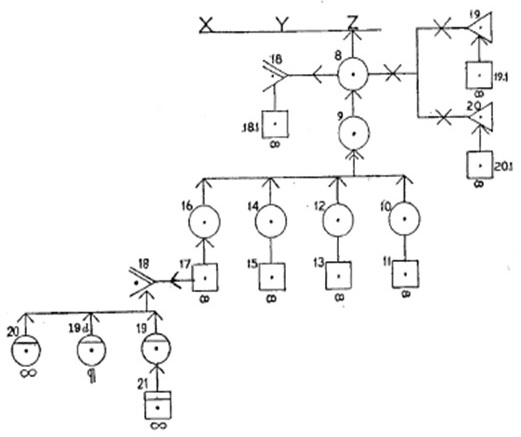
\includegraphics[scale=0.7]{img/wigmore.jpg}
\caption{A Wigmore chart\label{fig:wigmore}}
\end{figure}

\paragraph{The evaluation of an argument can depend on its subarguments.}Given an argumentative analysis of the case, one would like to know which conclusions follow, and which don't. We already discussed how arguments consisting of conflicts of reasons can be evaluated in this sense, when we discussed the role of exceptions, preferences and weighing (Section~\ref{sec:valueArgs}). More generally, the structure of a complex of arguments influences the evaluation of the arguments. In particular, the subarguments of a larger argument determine the evaluation of the whole. For an example, we go back to the argument in Figure~\ref{fig:arg2} (page~\pageref{fig:arg2}). There the witness report supported the intermediate conclusion that the suspect was at the crime scene, which in turn supported the conclusion that the suspect committed the crime. So there is an argument consisting of two steps. In the example, the first of these steps is attacked by a counterargument involving the lying of the witness. As a result of this attack, the argument to the intermediate conclusion that the suspect was at the crime scene breaks down and its conclusion does not follow. As a result, also the larger two-step argument no longer supports its conclusion, which hence does not follow. Since the one-step subargument does not successfully support the intermediate conclusion, also the whole two-step argument for the final conclusion does not successfully support its conclusion.

\paragraph{The evaluation of an argument can depend on chains of attacks.} When an argument is successfully attacked, it no longer successfully supports its conclusion. But attack can be chained, since the attack itself can be countered by a further attack. When an attack is successfully attacked, the original argument can become reinstated, in the sense that it again successfully supports its conclusion. Figure~\ref{fig:reinstatement} shows an example. A first witness, Witness $A$, reports that the suspect was at the crime scene. Given only this information, there is good reason to assume that the suspect was at the crime scene. However, there is a second witness, Witness $B$, who reports that Witness $A$ is lying. Given these two reasons, based on the witness reports by $A$ and $B$, it is no longer successfully supported that the suspect was at the crime scene. If now there is a third witness, Witness C, who reports that Witness B is lying, the attack is countered. Witness B is no longer believed, so there is no reason to conclude that Witness A is lying. As a result, A's report can again support its conclusion that the suspect was at the crime scene. The original argument based on A's report is reinstated. 

\paragraph{Conflicts between reasons can be addressed by exceptions, preferences and weighing.} The counterarguments to a reason that result from asking critical questions give rise to conflicts between reasons. Sometimes conflicts of reasons can be resolved in the sense that it can be determined which conclusions follow from the conflicting reasons. We distinguish three kinds of conflicts. 

In the first kind of conflicts between reasons, there is a reason attacked by an exclusionary reason, i.e., an attack of the undercutting kind that goes against the connection between the reason and its conclusion (cf. Section~\ref{sec:confArg}). This situation is shown at the top of Figure~\ref{fig:conflicts}: There is a witness reporting that the suspect was at the crime scene, but there is evidence that the witness is lying. 
%BV Done [ISN'T IT BETTER TO SAY THAT THERE IS EVIDENCE SUGGESTING THAT THE WITNESS IS LYING? ] 
In that case, the conclusion that the suspect was at the crime scene does not follow, since there is no supporting reason for it. The reason (the witness report itself) and the exception (the lying of the witness) both hold as they are assumptions. [DID YOU INTRODUCE THE IEDA OF ASSUMPTION ALREADY? IS IT NECESSARY?] In this situation of a reason with an undercutting attack by an exclusionary reason, the conflict of reasons is resolved by the exception expressed in the exclusionary reason. [NOT SURE I UNDERSTAND HOW THE CONFLICT IS RESOLVED HERE. THE UNDERCUTTING REASON WINS. OK. BUT HOW IS THIS A RESOLUTION OF THE CONFLICT?]

\begin{figure}[bt]
\centering
\documentclass[border=5mm,tikz]{standalone} 

\usepackage{amsmath}
% !TEX root=img/arguments_and_attack.tex

% \usetikzlibrary{external} 
% \tikzexternalize[prefix=tikz/] 

\usetikzlibrary{calc}
\usetikzlibrary{arrows}
\usetikzlibrary{arrows.meta}
\usetikzlibrary{decorations.markings}
% \usetikzlibrary{intersections}
\usetikzlibrary{fit}
\usetikzlibrary{shapes}
% \usetikzlibrary{trees}


\tikzset{
	every path/.style={thick},
	align=center,
	observed/.style={
		fill=black!20,
	},
	bn/.style={
		draw,
		ellipse,
		-{Triangle[angle=60:6pt 0]}
	},
	scn/.style={
		draw,
		rectangle,
		% signal,
		% signal from=west,
		% signal pointer angle=120,
		-{Triangle[angle=60:6pt 0]},
	},
	possibly/.style={dashed},
	arg/.style={
		draw,
		rectangle,
		-{Straight Barb[angle=60:6pt 0]}
	},
	attack/.style={
		-{Rays[width=10pt,length=10pt,sep=-3.9pt]}
	},
	pref/.style={
		draw,
		rectangle,
		-{Straight Barb[angle=60:6pt 0]}
	},
	subscn/.style={
		double,
		-{Triangle[angle=60:6pt 0]},
	},
	specific/.style={
		double,
		-{Stealth[angle=60:6pt 0]}
	},
}



\begin{document}
	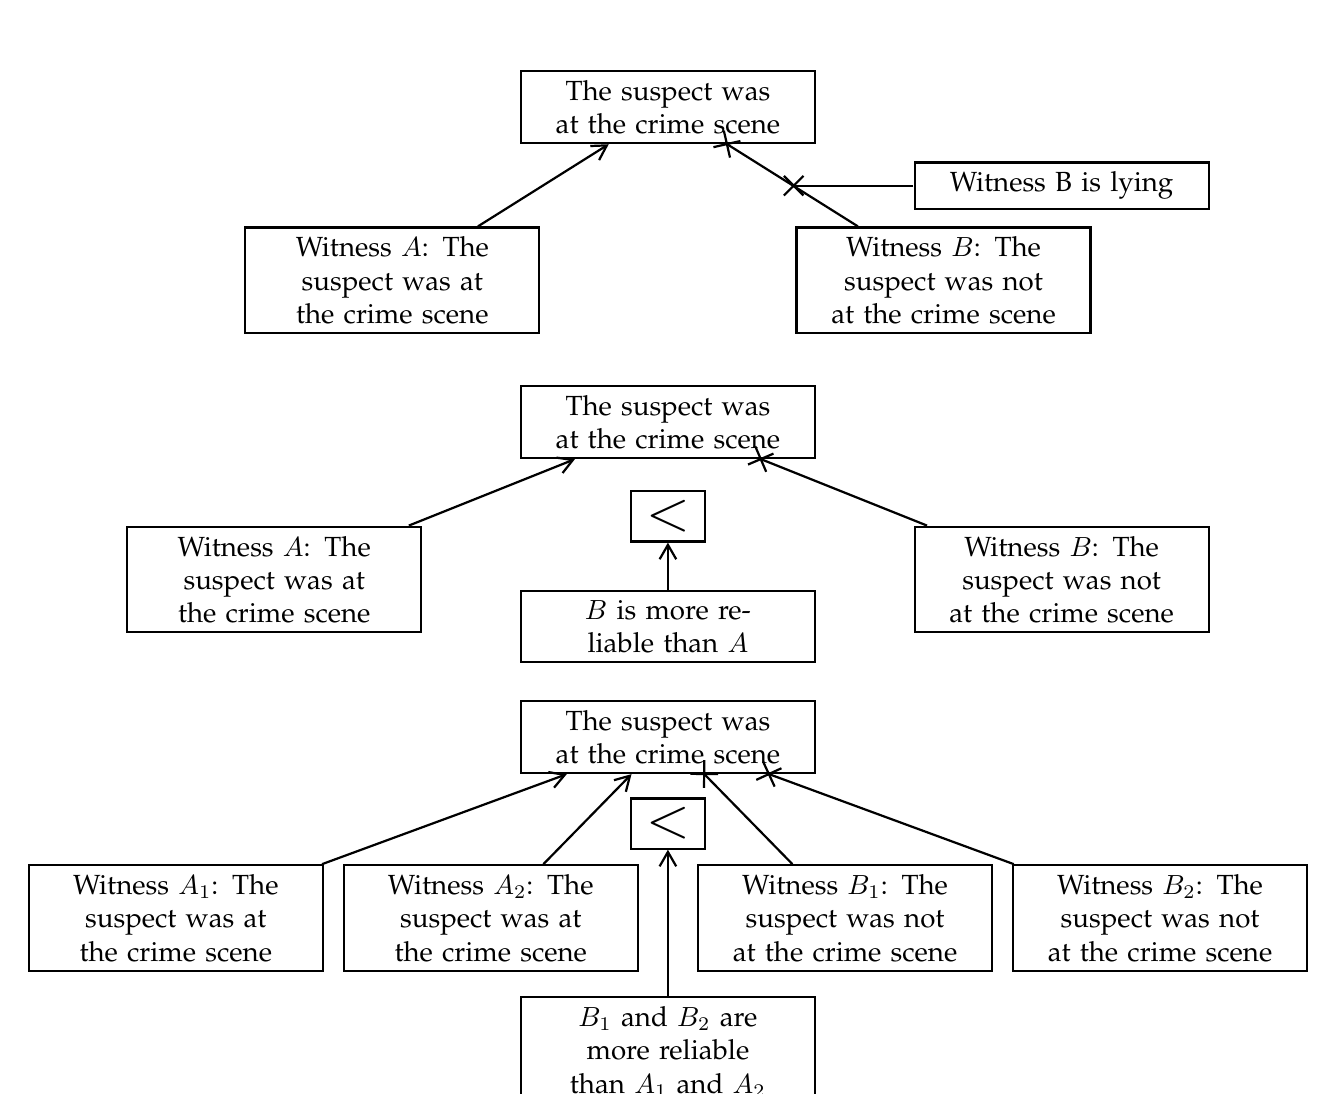
\begin{tikzpicture}[
		scnnode/.append style={text width=3cm},
		arg/.append style={text width=3.5cm},
		pref/.append style={text width=0.7cm},
	]
		\pgftransformxscale{5}
		\pgftransformyscale{2}

		\node[arg]     			(scene) at (0,0) {The suspect was at the crime scene};
		\node[arg] (witn) at (-0.7,-1.1) {Witness $A$: The suspect was at the crime scene};
		\node[arg] (witn2) at (0.7,-1.1) {Witness $B$: The suspect was not at the crime scene};

%		\node[arg] (witn) at (0,-1.1) {Witness: The suspect was at the crime scene};

		\node[arg] 					(lying) at (1,-0.5) {Witness B is lying};

		\draw[arg] 					(witn) -- (scene);
		\draw[attack] 					(witn2) -- (scene);
		\draw[attack] 			(lying) -- (0.32, -0.5);

%*********

		\node[arg]     			(scene) at (0,-2) {The suspect was at the crime scene};
		\node[arg] (witn) at (-1,-3) {Witness $A$: The suspect was at the crime scene};
		\node[arg] (witn2) at (1,-3) {Witness $B$: The suspect was not at the crime scene};

		\draw[arg] 					(witn) -- (scene);
		\draw[attack] 			(witn2) -- (scene);

		\node[pref] 				(pref) at (0,-2.6) 	{\huge $<$};
		\node[arg] 					(rel) at (0,-3.3) 		{$B$ is more reliable than $A$};

		\draw[arg] 					(rel) -- (pref);

%*********

		\node[arg]     			(scene) at (0,-4) {The suspect was at the crime scene};
		\node[arg] (witn) at (-1.25,-5.15) {Witness $A_1$: The suspect was at the crime scene};
		\node[arg] (witn2) at (-0.45,-5.15) {Witness $A_2$: The suspect was at the crime scene};
		\node[arg] (witn3) at (0.45,-5.15) {Witness $B_1$: The suspect was not at the crime scene};
		\node[arg] (witn4) at (1.25,-5.15) {Witness $B_2$: The suspect was not at the crime scene};

		\draw[arg] 					(witn) -- (scene);
		\draw[arg] 					(witn2) -- (scene);
		\draw[attack] 			(witn3) -- (scene);
		\draw[attack] 			(witn4) -- (scene);

		\node[pref] 				(pref2) at (0,-4.55) 	{\huge $<$};
		\node[arg] 					(outweigh) at (0,-6) 		{$B_1$ and $B_2$ are more reliable than $A_1$ and $A_2$};

		\draw[arg] 					(outweigh) -- (pref2);



	\end{tikzpicture}
\end{document}

\caption{Three kinds of conflicts and their resolution\label{fig:conflicts}}
\end{figure}

In the second kind of conflicts between reasons, there is one reason for a conclusion and another against the conclusion. For instance, there are two witnesses with opposite reports about whether the suspect was at the crime scene or not (see the middle of Figure~\ref{fig:conflicts}). This is an example of a rebutting attack (Section~\ref{sec:confArg}). The conflict of reasons is unresolved given only the reasons. Further information about the reasons is required to resolve the conflict. The resolution of such a conflict of reasons can be thought of as the preference of one over the other. A reason can be preferred over another, for instance when it is stronger. In the example, the preference (in the figure indicated by the $<$-sign) is argued for by the claim that one of the witnesses is more reliable than the other. In this case, the conclusion follows that the suspect was not at the crime scene, given this conflict of reasons and its resolution. 

The third kind of conflicts between reasons discussed here involves more than two reasons. For instance, there are more than two witnesses, with conflicting reports (Figure~\ref{fig:conflicts}, bottom). In the figure, both sides are supported by two witness reports. Resolving such a conflict can be thought of as a weighing of the reasons, generalizing the preference between two conflicting reasons. Again, it is concluded that the suspect was not at the crime scene, given this resolution of this conflict of reasons.

[I THOUGHT THE THREE TYPES OF CONFLICTS MIRRORED THE DISTINCTIONS BETWEEN UNDERCUTTING, REBUTTING AND UNDERMINING, 
BUT THE THIRD CONFLICT YOU DISCUSS HERE IS DIFFERENT FROM UNDERMINING. IS THIS INTENDED?]




\begin{figure}[bt]
\centering
\documentclass[border=5mm,tikz]{standalone} 

\usepackage{amsmath}
% !TEX root=img/arguments_and_attack.tex

% \usetikzlibrary{external} 
% \tikzexternalize[prefix=tikz/] 

\usetikzlibrary{calc}
\usetikzlibrary{arrows}
\usetikzlibrary{arrows.meta}
\usetikzlibrary{decorations.markings}
% \usetikzlibrary{intersections}
\usetikzlibrary{fit}
\usetikzlibrary{shapes}
% \usetikzlibrary{trees}


\tikzset{
	every path/.style={thick},
	align=center,
	observed/.style={
		fill=black!20,
	},
	bn/.style={
		draw,
		ellipse,
		-{Triangle[angle=60:6pt 0]}
	},
	scn/.style={
		draw,
		rectangle,
		% signal,
		% signal from=west,
		% signal pointer angle=120,
		-{Triangle[angle=60:6pt 0]},
	},
	possibly/.style={dashed},
	arg/.style={
		draw,
		rectangle,
		-{Straight Barb[angle=60:6pt 0]}
	},
	attack/.style={
		-{Rays[width=10pt,length=10pt,sep=-3.9pt]}
	},
	pref/.style={
		draw,
		rectangle,
		-{Straight Barb[angle=60:6pt 0]}
	},
	subscn/.style={
		double,
		-{Triangle[angle=60:6pt 0]},
	},
	specific/.style={
		double,
		-{Stealth[angle=60:6pt 0]}
	},
}



\begin{document}
	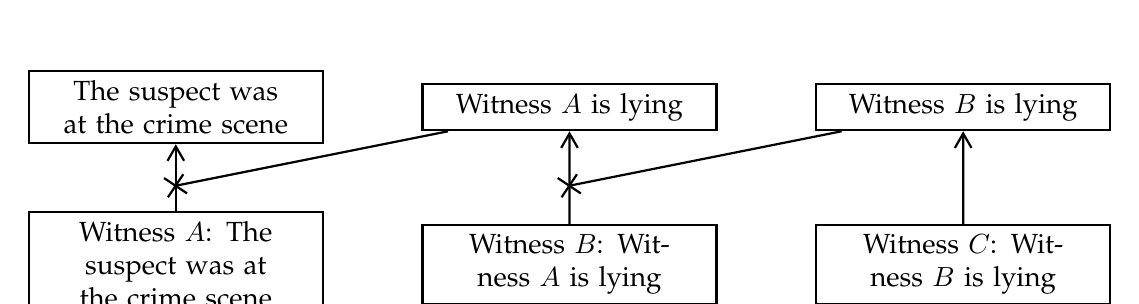
\begin{tikzpicture}[
		scnnode/.append style={text width=3cm},
		arg/.append style={text width=3.5cm},
	]
		\pgftransformxscale{5}
		\pgftransformyscale{2}

		\node[arg]     			(scene) at (0,-1) {The suspect was at the crime scene};
		\node[arg] (witn) at (0,-2) {Witness $A$: The suspect was at the crime scene};

		\draw[arg] 					(witn) -- (scene);

		\node[arg] 					(lying) at (1,-1) {Witness $A$ is lying};
		\node[arg] (witnB) at (1,-2) {Witness $B$: Witness $A$ is lying};

		\draw[attack] 			(lying) -- (0, -1.5);
		\draw[arg] 					(witnB) -- (lying);

		\node[arg] 					(lying2) at (2,-1) {Witness $B$ is lying};
		\node[arg] (witnC) at (2,-2) {Witness $C$: Witness $B$ is lying};

		\draw[attack] 			(lying2) -- (1, -1.5);
		\draw[arg] 					(witnC) -- (lying2);

	\end{tikzpicture}
\end{document}

\caption{Reinstatement\label{fig:reinstatement}}
\end{figure}


\paragraph{Further readings}
Pollock and his puzzles

The field of formal arg

Dung and his extensions

Arg evaluation software




%\paragraph{Inference to the best explanation (Allen/Pardo?)}

%\paragraph{WORRY: Confused about this one; why is it under coherence?) [Answer BV: Otherwise nothing remains here. ]}



\subsection{Probability}


\paragraph{Independent items of evidence can be combined by multiplying the likelihood ratios}
%BV As yet I am confused by this section. Notsure what to think. Let's discuss. Some bits are of my thoughts are as follows. First black sentence: Multiplication requires something else than independence, namely independence given H and given -H. Also the numeric examples aren't so helpful or so it seems as they are rather artificial. And: Is the point about two LRs canceling out when multiplied what we want to say? Second black point: This seems to be not so helpful. Third black point: This is an example far away from the range of examples we have been focusing on. Should this not be about combining two (or more) pieces of evidence and supporting two (or more) coherent events, aka scenarios?

In a criminal case, there may more than one piece of evidence, for example, 
there may be an eyewitness testimony and a DNA match. 
Suppose $P(\textit{guilt}| \textit{testimony})=0.7$
and $P(\textit{guilt} | \textit{match})=0.7$. What is the probability 
$P(\textit{guilt}| \textit{testimony} \wedge \textit{match})$ resulting 
from combing the two pieces of evidence? It would be a mistake to say that, assuming that 
the two items of evidence are independent, $P(\textit{guilt}| \textit{match} \wedge \textit{testimony})$ equals 
$0.7\times 0.7=0.49$. %How can  $P(\textit{guilt}| \textit{match}, \textit{testimony})$ be lower than  
%$P(\textit{guilt}| \textit{testimony})$ or $P(\textit{guilt}| \textit{match})$? 
The combination of two pieces of evidence, each favoring guilt to some extent, should strengthen the case for guilt, 
not weaken it. Observe that 
 %
\[\frac{P(\textit{guilt} | \textit{match}\wedge \textit{testimony})}{P(\neg \textit{guilt} | \textit{match}\wedge \textit{testimony})}=\frac{P(\textit{match}\wedge \textit{testimony} | \textit{guilt})}{P(\textit{match}\wedge \textit{testimony} | \neg \textit{guilt})}\times \frac{P(\textit{guilt})}{P(\neg \textit{guilt})},\]
 %
 and if \textit{match} and \textit{testimony} are independent, conditional on \textit{guilt}, then 
  %
\[\frac{P(\textit{match}\wedge \textit{testimony} | \textit{guilt})}{P(\textit{match}\wedge \textit{testimony} | \neg \textit{guilt})}=\frac{P(\textit{match}| \textit{guilt})}{P(\textit{match}|\neg \textit{guilt})}\times\frac{P(\textit{testimony} | \textit{guilt})}{P(\textit{testimony} | \neg \textit{guilt})}.\]
%
%or more succinctly,
%
%\[LR12 = LR1 \times LR2.\]
 %
%So, putting everything together,
 %
 %\[\frac{P(\textit{guilt} | \textit{match}, \textit{testimony})}{P(\neg \textit{guilt} | \textit{match}, \textit{testimony})}=LR1\times LR2\times \frac{P(\textit{guilt})}{P(\neg \textit{guilt})}.\]
 %
%
The point is that the likelihood ratios should be multiplied, not the probabilities of each hypothesis given the evidence. 
Suppose DNA evidence shows that the crime traces match with defendant, and 
the match has a likelihood ratio $\frac{P(\textit{match} | \textit{guilt})}{P(\textit{match}| \neg \textit{guilt})}$ of 36. 
Suppose the witness testimony favors the hypothesis of guilt and again has a likelihood ratio $\frac{P(\textit{testimony} | \textit{guilt})}{P(\textit{testimony}| \neg \textit{guilt})}$ of 36.
These numbers are purely illustrative. The combined evidential value of the two pieces of evidence is $36\times 36=1296$. 
This is a higher value than the two pieces of evidence considered separately, so 
$P(\textit{guilt}| \textit{match} \wedge \textit{testimony})$ will be greater than $P(\textit{guilt}| \textit{match})$ 
or $P(\textit{guilt}| \textit{testimony})$ considered separately, as expected. 
 
Multiplying the likelihood ratios increases the evidential 
value if the likelihood ratios are greater than one, and decreases the evidential value if the likelihood ratio 
are lower than one. If one likelihood ratio is greater and the other lower than one, that is, 
one item of evidence favors the hypothesis and the other disfavors it, 
their combined evidential value will vary.  To illustrate, consider a case in which 
%two items of evidence, 
%intuitively, cancel one another out.  
there are two conflicting testimonies. 
One witness asserts that the defendant was around the scene of the 
crime when the crime was committed. This incriminating testimony 
favors the hypothesis of guilt, for example,
%
\[\frac{P(\textit{incriminating witness}| \textit{guilt})}{P(\textit{incriminating witness} | \neg \textit{guilt)}}=\frac{0.9}{0.1}=9,\]
%
where the numbers are purely illustrative. 
The other witness offers an alibi for the defendant and asserts that she was with the defendant 
during the time of the crime. The alibi disfavors the hypothesis of guilt, so that 
%
\[\frac{P(\textit{alibi}| \textit{guilt})}{P(\textit{alibi}| \neg \textit{guilt})}=\frac{0.1}{0.9}=1/9,\] 
%
where the numbers are, once again, purely illustrative. 
 %Suppose $G$ has a probability of 0.5, regardless of the two testimonies.
%Suppose, also, that the incriminating testimony brings the probability of $G$ to 0.9, whereas the alibi brings the probability of 
%$G$ to 0.1 (and thus brings the probability of $\neg G$ to 0.9). Each testimony has the \textit{same yet divergent impact} on 
%$P(G)$. The incriminating testimony raises the probability of $G$ while the alibi lowers the probability SC. 
%They each do so to the same extent but in opposite directions. 
Absent further information about the trustworthiness of the testimonies, 
they should cancel one another. 
%The evidential value of each testimony  
%can be represented, in terms of likelihood ratios, 
%as follows:
%
%\[LR1=\frac{P(W1| G)}{P(W1|\neg G)}=\frac{0.9}{0.1}=9 \text{ and } LR2=\frac{P(W2|G)}{P(W2|\neg G)}=\frac{0.1}{0.9}=\frac{1}{9}.\]
%
The combined evidential value of the two testimonies is null, as expected, for
%
\[\frac{P(\textit{alibi}|  \textit{guilt})}{P(\textit{alibi}  \neg \textit{guilt})}\times \frac{P(\textit{incriminating witness}| \textit{guilt} )}{P(\textit{incriminating witness}| \neg\textit{guilt})}=9\times \frac{1}{9}=1.\] 
%
The multiplication of the likelihood ratios as a procedure to combine items of evidence 
can be used for more than two items of evidence. 
Assuming independence, the general 
formula is as follows:
%
\[LR_1\times \dots \times LR_k,\]
%
where $LR_i=\frac{P(E_i | H)}{P(E_i | \neg H)}$, for $i\in \{1, \dots, k\}$, and $H$ is the hypothesis of interest.

\paragraph{Items of evidence can be combined 
even if they are not independent}

So far we have assumed that the items of evidence to be combined are independent, 
conditional on guilt or on whatever hypothesis of interest. 
%More precisely, for the case of two items of evidence, 
%
%\[ \text{$E_1$ and $E_2$ are independent, conditional on $H$, iff $P(E_1 | H)= P(E_2 | E_1 \wedge H)$ }\]
%
If this assumption is dispensed with, the combined likelihood ratio is no longer the simple 
multiplication of the individual likelihood ratios, 
but rather, it becomes:
%
\[\frac{P(E_1\wedge E_2 | H)}{P(E_1\wedge E_2 | \neg H)}=\frac{P(E_1| H)}{P(E_1| \neg H)}\times \frac{P(E_2 | E_1\wedge H)}{P(E_2| E_1\wedge \neg H)},\]
%
and for more than two items of non independent evidence, the formula becomes:
%
\[\frac{P(E_1\wedge \dots \wedge E_k | H)}{P(E_1\wedge \dots \wedge E_k | \neg H)}=\frac{P(E_1| H)}{P(E_1| \neg H)} \times \dots \times \frac{P(E_k | E_1  \wedge \dots \wedge E_{k-1} \wedge H)}{P(E_k| E_1 \wedge \dots \wedge E_{k-1} \wedge \neg H)} .\]




\paragraph{Different items of evidence for different hypotheses can also be combined}

Another assumption that can be dispensed with is that the items of evidence favor or disfavor the \textit{same} hypothesis. % This assumption can be relaxed. 
Suppose a DNA match links the defendant to the crime scene, while an email written by the defendant indicates 
that he had a plan to kill the victim. Each of these item of evidence support a different hypothesis, abbreviated
 \textit{contact} and (\textit{plan}.
Suppose now $P( \textit{contact} | \textit{match})= 0.8$ and $P(\textit{plan} | \neg \textit{email})=0.8$. It is tempting 
to say that if the two hypothesis are independent, by the product rule, the probability of both hypotheses taken 
as a conjunction will be $0.8\times 0.8=0.64$, which is lower than the probability 
of each hypothesis considered separately.
%, as follows:
%
 %\[ \begin{array} {lcl } 
%P( \textit{contact} \wedge \textit{plan} | \textit{match} \wedge \textit{email})
 %& = & P( \textit{contact} | \textit{match}) \times 
%P(\textit{plan} |  \textit{email}) \\ 
 % & = & 0.9  \times  0.9\\
   % & = & 0.81
     % \end{array} \]
%
In general, by increasing the number of conjuncts, 
the probability of their conjunction can be made arbitrarily low. 
Paradoxically, it would seem that even if each conjunct has 
a high probability on the available evidence, their conjunction may have 
a very low probability given the evidence combined. 
This is known as the conjunction paradox. %But, the reasoning behind the conjunction paradox is mistaken. 

To deflect the paradox, observe that:
 %
\[ \frac{P(\textit{contact}\wedge \textit{plan} | \textit{match} \wedge \textit{email})}{P(\neg (\textit{contact} \wedge \textit{plan}) |  \textit{match} \wedge \textit{email})} 
=
\frac{P(\textit{match} \wedge \textit{email} | \textit{contact}\wedge \textit{plan})}{P(\textit{match} \wedge \textit{email} | \neg (\textit{contact} \wedge \textit{plan}))}
\times
\frac{P(\textit{contact}\wedge \textit{plan})}{P(\neg (\textit{contact} \wedge \textit{plan}))}
.\]
%
 Assuming that the two items of evidence are independent, conditional on 
 the hypothesis of interest, and assuming that the two hypotheses are also independent, we have:
 %
 \begin{eqnarray*}
 \frac{P(\textit{match} \wedge \textit{email} | \textit{contact}\wedge \textit{plan})}{P(\textit{match} \wedge \textit{email} | \neg (\textit{contact} \wedge \textit{plan}))}  
 & = &  \frac{P(\textit{match} | \textit{contact}\wedge \textit{plan})}{P(\textit{match} | \neg (\textit{contact} \wedge \textit{plan}))}  \times 
 \frac{P( \textit{email} | \textit{contact}\wedge \textit{plan})}{P(\textit{email} | \neg (\textit{contact} \wedge \textit{plan}))}  \notag\\ 
 && \notag\\
 & = & \frac{P(\textit{match} | \textit{contact})}{P(\textit{match} | \neg \textit{contact})}  \times  
 \frac{P( \textit{email} | \textit{plan})}{P(\textit{email} | \neg \textit{plan})}  \notag\\
 \end{eqnarray*}
%
Once again, the likelihood ratios, not the 
probabilities of each hypothesis, should be multiplied.  
Suppose, for the sake of argument, the evidential value of the DNA match in favor 
of the hypothesis \textit{contact}, 
and the evidential value of the defendant's email in favor of 
the hypothesis \textit{plan}, are as follows:
%
\[\frac{P(\textit{match}| \textit{contact})}{P(\textit{match} | \neg \textit{contact})}=36 \text{ and } \frac{P(\textit{email}| \textit{plan})}{P(\textit{email}| \neg \textit{plan})}=36\]
%
where the numbers are, as usual, illustrative. The combined evidential value of \textit{match} and \textit{email} 
in favor of the overall hypothesis, including \textit{contact} and \textit{plan}, is $36\times 36 = 1296$, so 
 
 %
 %\[
  \begin{eqnarray*} % {lcccc } 
 \frac{P(\textit{contact}\wedge \textit{plan} | \textit{match} \wedge \textit{email})}{P(\neg (\textit{contact} \wedge \textit{plan}) |  \textit{match} \wedge \textit{email})} 
 & = & 1296  \times 
\frac{P(\textit{contact}\wedge \textit{plan})}{P(\neg (\textit{contact} \wedge \textit{plan}))} \\ 
  \end{eqnarray*} 
  %\]
  %
  
  \noindent
For the value of the ratio $\frac{P(\textit{contact}\wedge \textit{plan})}{P(\neg (\textit{contact} \wedge \textit{plan}))}$, assume that 
%
\[\frac{P(\textit{contact})}{P(\neg \textit{contact})}=0.1/0.9 \text{ and } \frac{P(\textit{plan})}{P(\neg \textit{plan})}=0.1/0.9.\footnote{These assumptions are coherent with our earlier ones, 
so that%
 \[ \begin{array} {ccccc } 
 \frac{P(\textit{contact} | \textit{match})}{P(\neg \textit{contact} |  \textit{match})} 
 & = &  \frac{P(\textit{match} | \textit{contact})}{P(\textit{match} | \neg \textit{contact})} & \times &
 \frac{P(\textit{contact})}{P(\neg \textit{contact})} \\ 
 &&&&\\
 0.8/0.2 & = &  36 & \times &  0.1/0.9
   \end{array} \]
   %
and also
%
 \[ \begin{array} {ccccc } 
 \frac{P(\textit{plan} | \textit{email})}{P(\neg \textit{plan} |  \textit{email})} 
 & = &  \frac{P(\textit{email} | \textit{plan})}{P(\textit{email} | \neg \textit{plan})} & \times &
 \frac{P(\textit{plan})}{P(\neg \textit{plan})} \\ 
 &&&&\\
 0.8/0.2 & = &  36 & \times &  0.1/0.9
   \end{array} \]
%
}\]
%
Now, putting everything together, we get
 
 %\[ 
 \begin{eqnarray*} %{ccccc } 
 \frac{P(\textit{contact}\wedge \textit{plan} | \textit{match} \wedge \textit{email})}{P(\neg (\textit{contact} \wedge \textit{plan}) |  \textit{match} \wedge \textit{email})} 
 & = & \frac{P(\textit{match} \wedge \textit{email} | \textit{contact}\wedge \textit{plan})}{P(\textit{match} \wedge \textit{email} | \neg (\textit{contact} \wedge \textit{plan}))}  \times 
\frac{P(\textit{contact}\wedge \textit{plan})}{P(\neg (\textit{contact} \wedge \textit{plan}))} \\ 
 &&\\
0.93/0.07 & = & 1296  \times  \frac{0.1\times 0.1}{1-(0.1\times 0.1)}
 \end{eqnarray*} %\]
  %

So, the $P(\textit{contact}\wedge \textit{plan} | \textit{match} \wedge \textit{email})$ turns out to 
be higher, albeit somewhat only slightly, than $P(\textit{contact}| \textit{match})$ or
 $P(\textit{plan} | \textit{email})$. By combing different items of evidence and different hypotheses, the probability of the conjunction 
need not be lower than the probability of each conjunct, \textit{contra} the conjunction of paradox. 


\paragraph{Further readings}
The conjunction paradox \citep{cohen1977} and a response \citep{dawid1987}. 
Coherence and probability \citep{bovensHartman2003}.
Bayesian networks \citep{taroniEtal2006}. Probabilistic 
analysis of an entire legal case \citep{kadaneSchum1996}.
On the use of probability in law \citep{fenton2011}.






%\section{When can we convict?}
\section{Reasoning and Decision Making}
\label{sec:whenconv}
\label{sec:intexc}

%\subsection{Beyond a reasonable doubt}

So far we have focused on how the evidence can be evaluated and combined, and how inferences can be drawn. 
This does not take place in vacuum. 
The legal system contains rules for the discovery, admission and exclusion of the evidence. 
The legal system also contains 
procedures and guarantees available to defendants. In most countries, for example, criminal defendants enjoy 
the right to cross examine their accusers and scrutinize the evidence presented against them, and all defendants are 
presumed innocent until proven guilty. 
%During the dialectical confrontation between two parties, each defending their side of the case, 
%the role of judge is sometimes that of a mere arbiter or an active participant as well. 
Once the evidence has been introduced at trial, examined and cross examined, it comes a time when the fact finders, either a 
trained judge or a group of lay jurors, must reason from the evidence, reach a conclusion and decide 
whether to convict or acquit the defendant. 
%The decision should be based on the evidence presented 
%and the law governing the case, not human feelings, but this leaves two important questions unanswered. The first is how  
%the reasoning from the evidence to the conclusion should be conducted. The second concerns the appropriate standard that 
%should govern the decision. In continental Europe until the 18th century, an elaborate system of legal arithmetic 
%was in place, dividing legal proofs in full and half proofs and detailing how proofs could be added to one another. REFERENCES. 
%With the Enlightenment, however, free proof gained momentum and the system of legal arithmetic fell in disrepute.

%Currently, there is no strict regulation of how the fact finders should reason or 
%reach conclusions on the basis of the evidence. However, 
The decision criterion is defined by law 
and consists of a standard of proof, sometimes also called burden of persuasion. This is not to be confused with 
the burden of proof, which includes the burden of persuasion as well as the burden of production.
%The standard of proof identifies, in a somewhat verbally imprecise manner, 
%how strong the evidence should be for warranting a finding of criminal liability. Failure to meet the standard of proof must 
%result in an acquittal. 
The criterion for criminal cases in common law countries is 
\textit{proof beyond a reasonable doubt}, and a similar criterion exists outside the common law.
 If the decision makers are persuaded of the defendant's guilt beyond a reasonable doubt, 
 they should convict, or else they should acquit.  

In Commonwealth v.\ Massachusetts Webster (1850), 
proof beyond a reasonable doubt is equated to 
`reasonable and moral certainty'. In R.\ v.\ Lifchus (1997),  the Supreme Court of Canada writes that 
the `the standard of proof beyond a reasonable 
doubt is inextricably intertwined with \dots 
the presumption of innocence', that it is connected with `the evidence or  
absence of evidence', and also that `it does not involve proof to an absolute certainty' and so 
`it is not proof beyond any doubt' (335). 
Explanations abound in the case law. And yet, it is unclear 
whether they improve our understudying. The US Supreme Court might have been right when, in Holland v.\ United States (1954), 348 U.S. 121, 
it wrote that that `attempts to explain the term ``reasonable doubt'' do not result in making it any clearer' (140).
 
 
The three frameworks we considered---probability, arguments and narratives---can be used to characterize 
more precisely the standard of proof, although they are not immune from shortcomings either, 
as we shall soon see.


\paragraph{Further readings}
Evidence law manuals  \citep{fisher2008,  mendez2008}. 
Criminal Procedure manuals \citep{allenEtAl2011}.
Character evidence and its exclusion \citep{redmayne2015}.
Free proof, legal arithmetic and rules of weight.
 

 
 




\subsection{Probability}


\paragraph{The guilt probability is estimated by weighing  the evidence through Bayes' theorem}

 On the probabilistic framework, the goal is to estimate the probability of the defendant's guilt based 
 on all the available evidence. The estimation begins with the lowest possible value 
for the guilt probability, prior to considering any evidence. As more evidence is presented, the guilt probability 
moves upwards or downward depending on whether the evidence is incriminating or exculpatory. 
When all the evidence is considered, a final guilt probability value is 
reached, all things considered. This forms the basis for 
the decision to convict or acquit. 

The value of the guilt probability is arrived at by applying Bayes' theorem a 
repeated number of times and by plugging the values of the probabilities that are needed. 
Sometimes these probabilities are known because they are based on estimated frequencies, but sometimes 
they are not. For example, $P(G)$ is required to calculate $P(G|E)$. 
This is the probability of the defendant's guilt regardless of the evidence 
presented at trial. What should $P(G)$ be?
For technical reasons, it cannot be zero, but it also cannot be 50\% because 
of the presumption of innocent. Arguably, $P(G)$ should be relatively low, but how low?
This remains  hotly debated. 


\paragraph{The decision criterion is a guilt probability threshold}

In probabilistic terms, proof of guilt beyond a reasonable doubt means 
that the defendant's \textit{probability of guilt}, given the evidence presented at trial, meets a 
threshold, say, $>$99\% or $>$99.9\%. 
%Consequently, a 
%doubt would be reasonable or unreasonable depending on a measurable probability.  
%
A numerical value for the threshold can be identified using expected utility theory. 
Let $c(CI)$ be the cost of convicting an innocent and $c(AG)$ the cost 
of acquitting a guilty defendant. For a conviction to be justified, the 
expected cost of convicting an innocent must be lower than the expected 
cost of acquitting an innocent, that is, 
%
\[ P(G|E) \times c(AG) >  [1-P(G|E)] \times c(CI) .\]
%
%The inequality represents a situation in which the expected cost resulting from convicting an innocent is lower than the expected cost
%resulting from a cutting a guilty defendant. Given the inevitable possibility of error, such a situation would be one in which 
%convicting is less costly than acquitting, so convicting is justified. Crucially, 
The inequality holds just in case 
%
\[ \frac{P(G|E)}{1- P(G|E)} > \frac{c(CI)}{c(AG)}.\]
%
%This formula gives a precise indication of how high the probability 
%of guilt must be to justify a guilty verdict, relative to the ratio between $D_i$ and $D_g$. 
%If we consider thatthe disutility of convicting an innocent is as harmful as the disutility of acquitting an innocent, 
%i.e., $D_g=D_i$---as it might be the case in a civil case---, the lower bound for $P_g$ must be at least $\frac{1} {2}$. 
Suppose $ \frac{c(CI)}{c(AG)}=\frac{99}{1}$, as might be more appropriate in a criminal 
case in which the conviction of an innocent defendant is regarded as far worse than the acquittal of a guilty defendant.
Then, the inequality hold only if $P(G)$ meets the threshold 99\%.
More complicated models are also possible, but the basic idea is that the probability 
required for a conviction is a function of weighing the 
costs that would result from an erroneous decision. 

%MENTION PROOF PARADOXES HERE. 

\paragraph{The probabilistic framework can be thought of as an idealization}

The characterization is simple, crisp and elegant, but a too literal interpretation of it is problematic.  If a probabilistic threshold is understood as a criterion which the decision makers 
 should mechanically apply whenever they confront the decision to convict or acquit, two difficulties arise. The first difficulty is that assigning a probability value to guilt itself might not be feasible. As seen earlier, the starting probability $P(G)$ cannot be easily determined, 
and even if this value could be known, other probability values might remain unknown. One solution here is that instead 
 of aiming for a unique guilt probability, we can simply aim for an interval of admissible probabilities given the evidence. 
 More generally, the estimation of the probability of guilt can be viewed as an idealized process, a regulative ideal which can improve the precision of legal reasoning. 
In this spirit, setting a probabilistic criterion for criminal convictions would only be a way 
to theorize about the meaning and ideal of the criminal standard of proof. 

Another problem with the probabilistic characterization 
is that it does not take into account the so-called weight of the evidence, that is, whether the evidential basis contains all the evidence 
in the case or just a partial subset of the evidence. The guilt probability will vary dramatically 
depending on the evidence that is used to estimate it. It is tempting to suggest that the guilt probability must be based on a body 
of evidence that is complete, or at least as complete as reasonably possible. And yet, it is unclear how to characterize this notion.

\paragraph{Further readings}

Probabilistic accounts of the burden of proof
\citep{kaplan1968, kaye1986, kaye1999, hamer2004, cheng2013}.
Critique of probabilistic accounts \citep{cohen1977, nesson79, thomson86, stein05, ho08, pardoAllen2008, haack2011}.
On the question whether the threshold should be variable \citep{kaplow2012, picinali2013}.
The problem of priors \citep{finkelsteinFairley1970, friedman2000}.
A critique of the proof beyond a reasonable doubt  
as understood in the law \citep{laudan2006}.
History of beyond a reasonable doubt standard 
\citep{shapiro1991, whitman2008}. Other measures, weight, resiliency and completeness 
of the evidence \citep{kaye1999, stein05}.




\subsection{Arguments}


\paragraph{Arguments and countearguments can be represent in argument graphs}

In a court of law, the prosecutor or plaintiff puts forward a claim and offers supporting arguments. The opposing parts responds by offering counterarguments. The dialectical process can be complex. There are different counterarguments: undermining,  undercutting and rebutting. The process is complex also because it can iterated. 
An argument can be attacked by a counteargument, and the latter in turn can be attached by a further counterargument. And so on. 
When the dialectical process reaches an equilibrium point and the opposing parties have nothing more to contribute, 
the status of a claim and its supporting argument can be assessed. 

On the argument based 
framework, the goal is to consider all the available arguments, by representing them in a comprehensive argumentation graph that 
keeps track of the relations of support and attack between arguments. The two competing theories of the cases, the prosecutor's and the defense's theory, will each
be supported by a set of arguments. The argument framework, through the aid of argument graphs, allow us to 
compare the relative strength of the arguments in favor of one side of the case or the other. This comparison of the argumentative strength of the two sides 
forms the basis for the trial decision.


\paragraph{Defeating all counterarguments is the criterion for meeting the standard of proof}

In order to establish the defendant's guilt beyond a reasonable doubt, all counterarguments 
to the contrary must be responded, or in other words, all the attacks against the argument for guilt must be 
defeated. Now, whether a counteargument or an attack is defeated 
is not always an all or nothing affair. It is often a matter of degrees. 
If the argument for guilt is slightly stronger than all its counterarguments, this would not be enough yet. 
To meet the demands of the standard of proof beyond a reasonable doubt, an argument must be significantly 
stronger than all its counterarguments. On the other hand, defeating all its counterarguments with absolute certainty would be too much to expect. 
So, more realistically, all counterattacks must be defeated in an almost definitive way. Here, it seems, we need 
to reintroduce some threshold, even though not in an explicitly probabilistic or numerical way. 


\paragraph{The argumentation framework is intuitive but lacks normative force}


The argumentation framework is rather realistic. The dialectic between arguments and 
counterarguments effectively take place in court, and the idea that meeting the standard of proof requires to answer all 
counterargument against guilt is natural enough. A problem is that if the opposing party puts forward no counterarguments, meeting the standard of proof would be effortless. A possible response here is that the counterarguments must be all the counterarguments which a reasonable objector could in principle put forward, not just 
the counterarguments that in fact are put forward. %Here again we see we must recourse to some dose of idealization or abstraction. 

Another problem consists in identifying the threshold. While the probability based account can identify a specific probability threshold, 
at least in theory, by applying the principle of expected utility theory, the argumentation based framework cannot. 
How could the principle of expected utility theory be applied to the argument framework as well?



\paragraph{Further readings}
Carneades model \citep{gordonEtal2007, gordon2009}.
Justified argument model \citep{prakkenSartor2007, prakken2009}.



\subsection{Scenarios}


\paragraph{Competing scenarios must be compared and evaluated}

On the narrative framework, the two parties will put forward competing scenarios, at least two or possibly more than two. This is partly problematic because in a criminal case, the defense does not have the burden of proof. So it might well be that the defense puts forward a scenario that weakens the prosecutor's scenario, but that is not 
a scenario that proves innocence. Be that as it may, the various competing scenarios will be evaluated along the different criteria we identified, such as, consistency with the evidence, explanatory power, plausibility, cohesiveness, etc. The question arises, which scenario should be selected among the competitors?



\paragraph{The best scenario is the rule of decision}

We can picture the process of evaluation of the competing scenario as a process of elimination. 
At the beginning, several scenarios are viable, but as more evidence is considered and the scrutiny of each scenario continues,
fewer scenarios will survive. The goal would be to select one scenario, or at least a limited set of scenarios, so that 
the answer to the question `guilty or not?' would be univocal. On this picture, a scenario meets the demands of the standard 
of proof whenever it is the \textit{only} scenario left.

But, once again, we confront a recurrent problem. The selection of one scenario is not always an all or nothing affair.
The term `abduction' or the expression `inference to the best explanation' is sometimes used in this context. The basic idea if that, when confronted 
with two or more competing scenarios, the best explanation must be chosen. The notion of `best explanation' here is wide ranging. It includes criteria such as 
consistency with the evidence, explanatory power (predictive power and causal fit), evidential support, plausibility, completeness, etc. 
Other criteria might also play a role, such the simplicity of the scenario.  So, the best explanation is the scenario that fares 
better on some combination of these criteria. This is a matter of degrees. The scenarios get higher 
or lower scores relative to the applicable evaluation criteria. The scenario that gets the best score, and that 
meets a suitable threshold level, should be selected. 





\paragraph{The process of scenario selection is underspecified}

The process of scenario selection resembles how jurors reason in trial proceedings, whereas despite its 
clear mathematical underpinnings, it is hard to relate probability to judicial proceedings: jurors do not 
naturally quantify guilt, and it is difficult to quantify it even if we wanted to. Still, a problem with the scenario approach is that 
the method by which a scenario is selected is not be transparent. The different criteria, such as consistency, explanatory power, coherence etc.\ 
can pull the decision makers in opposite directions. For example, a scenario might be better in terms of explanatory power, while another scenario might 
be more plausible. What to do, then? One might wonder whether the criterion for the best scenario should simply be this:
the most probable scenario which meets a sufficiently high probability threshold. If so, this would not be very 
different from the probability account. 

\paragraph{Further readings}

Inference to the best explanation \citep{lipton1991}.
Application of inference to the best explanation 
to legal reasoning \citep{pardoAllen2008}. 
Narrative based account of proof beyond a 
reasonable doubt \citep{allen2010, allenStein2013}.
















\section{Summary and conclusion}



There is room for studying the further integration of the three normative frameworks.







%\bibliographystyle{spbasic}
\bibliographystyle{plainnat}	
%\bibliography{dissertation,cumulative}
\bibliography{cumulative}






\end{document}

